% Asset preview project (NOT the paper). Compiles on Overleaf with pdfLaTeX + BibTeX.
\documentclass[conference]{IEEEtran}
\usepackage[T1]{fontenc}
\usepackage{graphicx}
\usepackage{booktabs}
\usepackage{amsmath}
\usepackage{url}
\usepackage{cite}
% Figure captions as macros: % Figure captions as macros: % Figure captions as macros: \input{captions_figures} then use e.g. \CapFigSystemArchitecture
% Generated by paper_assets/scripts/make_docs.py
\newcommand{\CapFigZeroOneSystemArchitecture}{Overall architecture of the proposed system. The offline pipeline (top) trains a Random Forest on Backblaze SMART data (1 April -- 24 May 2019) and writes one prior-corrected 7-day failure score per drive-day for 1--23 June. Only these scores enter the trace-driven CloudSim simulation (bottom), where a risk classifier and an adaptive checkpoint scheduler set each host's checkpoint interval. Failure times come from a separate trace that only the failure injector reads; failure labels are never passed to the simulator. Orange borders: custom components; grey: native CloudSim.}
\newcommand{\CapFigZeroTwoMlPipeline}{Random Forest prediction pipeline. Steps 1--8 run offline; step 9 (risk classification) is applied inside the simulator. Labels use a 7-day horizon: a drive-day is positive if the drive records a failure on day t+1 to t+7. The tier boundaries are the 90th and 99th percentiles of validation scores and were not tuned on test data.}
\newcommand{\CapFigZeroThreeAdaptiveCheckpointing}{Adaptive checkpoint scheduling (policy E3). The Random Forest supplies only a risk score. A fixed classifier maps the score to a tier, and the scheduler maps the tier to a checkpoint interval $\tau$ relative to the baseline $T_0$. The table lists the resulting intervals for each $T_0$; the fixed policy E2 uses $\tau = T_0$ for every tier.}
\newcommand{\CapFigZeroFourCloudsimIntegration}{CloudSim integration and recovery architecture. Native CloudSim 3.0.3 entities (grey) are used unmodified. The custom broker runs each job as a chain of compute-segment cloudlets and writes each checkpoint as a 300 s cloudlet. On a host failure it moves the job to a spare host and restores from the last completed checkpoint. Each Backblaze drive is modelled as one host, and a recorded disk failure is treated as a host failure; this is a modelling assumption.}
\newcommand{\CapFigZeroFiveExecutionFlow}{End-to-end execution flow for one job. A job runs in compute segments that end at the next checkpoint due time, at midnight (when the daily risk tier may change) or at job end. A host failure interrupts the running segment or checkpoint write. The job then resumes on a spare host after $D + B = 180$ s: from its last completed checkpoint after a 300 s restore, or from zero if no checkpoint exists.}
\newcommand{\CapFigZeroSixExperimentalDesign}{Experimental design. In each scenario, all 11 policy configurations (E1, plus E2 and E3 at five baseline intervals $T_0$) run on all 56 shards with the identical workload, failure trace and risk trace, so comparisons are paired. The two load scenarios ($\rho = 0.9$ primary, $\rho = 1.0$ saturated sensitivity) have different workloads and are analysed separately.}
\newcommand{\CapGZeroOneRfRocCurve}{ROC curve of the Random Forest on the 1--23 June test set (2,544,754 drive-days, 997 positives). (a) Full curve, AUC = 0.804. (b) The same curve with a logarithmic FPR axis; markers show recall at 0.1\,\% FPR (16.0\,\%) and 1\,\% FPR (37.3\,\%).}
\newcommand{\CapGZeroTwoRfPrecisionRecallCurve}{Precision--recall curve on the June test set (PR-AUC = 0.0337, about 86 times the 0.039\,\% prevalence; log-scaled precision axis). The marker shows the alarm threshold 0.01368 chosen by maximum F1 on validation: precision 4.3\,\%, recall 20.7\,\%.}
\newcommand{\CapGZeroThreeRfConfusionMatrix}{Confusion matrix on the June test set at the validation-selected threshold ($p \ge 0.01368$). Shading shows the row-normalised rate. The model raises 4,597 false alarms for 206 true positives and misses 79\,\% of positive drive-days.}
\newcommand{\CapGZeroFourRfScoreDistribution}{Distribution of prior-corrected scores (log scale) for June drive-days with and without a failure in the next 7 days, each normalised to 100\,\%. Dotted lines mark the tier boundaries (0.000234, 0.001732) and the alarm threshold (0.01368). The two classes overlap substantially.}
\newcommand{\CapGZeroFiveRfFeatureImportance}{Top 15 features. (a) Mean decrease in impurity, final model. (b) Permutation importance (mean decrease in average precision $\pm$ s.d.) of the internal-validation model on a validation subsample. Reallocated-sector counts (SMART 5) dominate both rankings. Correlated features share importance, so the rankings should be read in groups.}
\newcommand{\CapGZeroSixOverheadVsTZeroRhoZeroNine}{Checkpoint overhead as a percentage of useful computation for fixed (E2) and RF-adaptive (E3) checkpointing at each baseline interval $T_0$, $\rho = 0.9$, all hosts (log scale; E1 has no overhead). Whiskers are 95\,\% host-clustered bootstrap CIs and are very narrow. E3 is lower at $T_0 \le 12$\,h and higher at 24--72\,h.}
\newcommand{\CapGZeroSevenLostWorkVsTZeroRhoZeroNine}{Lost computation caused by the 175 host failures, $\rho = 0.9$ (log scale). The dashed line shows no checkpointing (E1, 8,375\,h). Whiskers are 95\,\% bootstrap CIs; they are wide because they rest on 175 failure events.}
\newcommand{\CapGZeroEightDeadlineMissVsTZeroRhoZeroNine}{Deadline miss rate, $\rho = 0.9$. (a) All hosts: only E3 at $T_0 = 1$\,h misses an appreciable share (4.54\,\%). Every other E2/E3 configuration misses at most 0.015\,\%; value labels below 0.05\,\% are omitted. (b) The 175 failing hosts: E1 misses 19.8\,\%, and E3 at 1\,h misses 23.3\,\%. Whiskers are 95\,\% bootstrap CIs.}
\newcommand{\CapGZeroNineWastedTimeAllPoliciesRhoZeroNine}{Total wasted time (checkpoint overhead + lost work + interrupted checkpoint writes + recovery) as a percentage of useful computation, $\rho = 0.9$ (log scale). No checkpointing (E1) wastes the least overall (0.011\,\%). At these failure rates, checkpointing pays off by protecting the jobs that failures hit (Fig.~\ref{fig:deadline_rho09}b), not in aggregate efficiency.}
\newcommand{\CapGTenOverheadVsLostTradeoffRhoZeroNine}{Trade-off between overhead and lost computation, $\rho = 0.9$ (log--log). Each point is one policy at one $T_0$; labels are on the E2 points, and the E3 point for the same $T_0$ lies just below. E3 is lower on both axes at $T_0 \le 12$\,h; the 1\,h point carries a deadline penalty (Fig.~\ref{fig:deadline_rho09}). At 24 and 72\,h, E3 trades higher overhead for lower lost work. Whiskers: 95\,\% CIs of lost work.}
\newcommand{\CapGElevenCheckpointsPerJobRhoZeroNine}{Mean checkpoints per job, $\rho = 0.9$ (log scale). E3 writes fewer checkpoints than E2 at $T_0 \le 12$\,h, because 54\,\% of June host-days are LOW, and more at 24--72\,h.}
\newcommand{\CapGTwelvePairedEThreeVsETwoRhoZeroNine}{Paired E3 $-$ E2 differences at equal $T_0$, $\rho = 0.9$, all hosts: (a)--(c) relative to E2, (d) in percentage points. Intervals are 95\,\% host-clustered bootstrap CIs of the difference, rescaled by the E2 point estimate in (a)--(c). Filled markers: the interval excludes 0. Negative values favour E3. The intervals are not adjusted for multiple comparisons, and no significance is claimed.}
\newcommand{\CapGTwelvePairedEThreeVsETwoRhoOneZero}{Paired E3 $-$ E2 differences at equal $T_0$ under saturation, $\rho = 1.0$, all hosts. The format is the same as Fig.~\ref{fig:paired_rho09}. This experiment has a different workload from $\rho = 0.9$, so its effects are compared only in direction and size.}
\newcommand{\CapGThirteenDeadlineMissVsTZeroRhoOneZero}{Deadline miss rate under saturation, $\rho = 1.0$, all hosts. Without slack, checkpoint overhead becomes queueing delay: at $T_0 = 1$\,h, E2 misses 50.7\,\% of deadlines and E3 34.2\,\%; at 4\,h, 7.6\,\% versus 3.2\,\%. At 12\,h, E3 is worse (0.27\,\% versus 0.01\,\%).}
\newcommand{\CapGFourteenQueueingVsTZeroRhoOneZero}{Mean queueing delay per job, $\rho = 1.0$ (log scale). E3 reduces queueing at every $T_0$. The dashed line shows E1 (0.04\,h).}
\newcommand{\CapGFifteenLostWorkVsTZeroRhoOneZero}{Lost computation, $\rho = 1.0$ (log scale), with 95\,\% bootstrap CIs. The dashed line shows E1 (9,603\,h).}
\newcommand{\CapGSixteenFailingHostDeadlineMissBothRho}{Deadline miss rate on the 175 failing hosts, fixed (E2) versus adaptive (E3): (a) $\rho = 0.9$, (b) $\rho = 1.0$. Under saturation, E3's extra checkpoints on HIGH-tier hosts raise failing-host deadline misses at $T_0 \le 4$\,h (25.5\,\% versus 14.9\,\% at 4\,h), even though lost work falls. The two panels are separate experiments with different workloads.}
\newcommand{\CapGSeventeenTierOccupancy}{Share of June host-days in each risk tier, compared with the validation design target (90/9/1\,\%). June scores are shifted upward: only 54.1\,\% of host-days are LOW, and 6.6\,\% are HIGH. Failing hosts spend 52.3\,\% of their host-days in HIGH.}
\newcommand{\CapGEighteenFailuresByTier}{Risk tier in force at the instant of each of the 175 failures, identical across policies and scenarios: 110 HIGH, 38 MEDIUM and 27 LOW.}
\newcommand{\CapGNineteenLostWorkByTierRhoZeroNine}{Lost computation grouped by the tier in force at failure, $\rho = 0.9$ (log scale; point estimates). E3 sharply reduces lost work for failures in HIGH and has little effect in MEDIUM. It increases lost work for the 27 failures the model ranked LOW, where its interval is 2.65\,$T_0$.}
\newcommand{\CapGTwentyOverheadByTierRhoZeroNine}{Checkpoint overhead split by the tier in force when each checkpoint was written, $\rho = 0.9$, all hosts, indexed to the E2 total at the same $T_0$ (= 100). E3 cuts LOW-tier overhead and spends much of the saving on HIGH-tier checkpoints. At $T_0 = 72$\,h the LOW interval (190.8\,h) exceeds the longest job (168\,h), so E3 writes almost no LOW-tier checkpoints (0.2\,\% of its checkpoints).}
 then use e.g. \CapFigSystemArchitecture
% Generated by paper_assets/scripts/make_docs.py
\newcommand{\CapFigZeroOneSystemArchitecture}{Overall architecture of the proposed system. The offline pipeline (top) trains a Random Forest on Backblaze SMART data (1 April -- 24 May 2019) and writes one prior-corrected 7-day failure score per drive-day for 1--23 June. Only these scores enter the trace-driven CloudSim simulation (bottom), where a risk classifier and an adaptive checkpoint scheduler set each host's checkpoint interval. Failure times come from a separate trace that only the failure injector reads; failure labels are never passed to the simulator. Orange borders: custom components; grey: native CloudSim.}
\newcommand{\CapFigZeroTwoMlPipeline}{Random Forest prediction pipeline. Steps 1--8 run offline; step 9 (risk classification) is applied inside the simulator. Labels use a 7-day horizon: a drive-day is positive if the drive records a failure on day t+1 to t+7. The tier boundaries are the 90th and 99th percentiles of validation scores and were not tuned on test data.}
\newcommand{\CapFigZeroThreeAdaptiveCheckpointing}{Adaptive checkpoint scheduling (policy E3). The Random Forest supplies only a risk score. A fixed classifier maps the score to a tier, and the scheduler maps the tier to a checkpoint interval $\tau$ relative to the baseline $T_0$. The table lists the resulting intervals for each $T_0$; the fixed policy E2 uses $\tau = T_0$ for every tier.}
\newcommand{\CapFigZeroFourCloudsimIntegration}{CloudSim integration and recovery architecture. Native CloudSim 3.0.3 entities (grey) are used unmodified. The custom broker runs each job as a chain of compute-segment cloudlets and writes each checkpoint as a 300 s cloudlet. On a host failure it moves the job to a spare host and restores from the last completed checkpoint. Each Backblaze drive is modelled as one host, and a recorded disk failure is treated as a host failure; this is a modelling assumption.}
\newcommand{\CapFigZeroFiveExecutionFlow}{End-to-end execution flow for one job. A job runs in compute segments that end at the next checkpoint due time, at midnight (when the daily risk tier may change) or at job end. A host failure interrupts the running segment or checkpoint write. The job then resumes on a spare host after $D + B = 180$ s: from its last completed checkpoint after a 300 s restore, or from zero if no checkpoint exists.}
\newcommand{\CapFigZeroSixExperimentalDesign}{Experimental design. In each scenario, all 11 policy configurations (E1, plus E2 and E3 at five baseline intervals $T_0$) run on all 56 shards with the identical workload, failure trace and risk trace, so comparisons are paired. The two load scenarios ($\rho = 0.9$ primary, $\rho = 1.0$ saturated sensitivity) have different workloads and are analysed separately.}
\newcommand{\CapGZeroOneRfRocCurve}{ROC curve of the Random Forest on the 1--23 June test set (2,544,754 drive-days, 997 positives). (a) Full curve, AUC = 0.804. (b) The same curve with a logarithmic FPR axis; markers show recall at 0.1\,\% FPR (16.0\,\%) and 1\,\% FPR (37.3\,\%).}
\newcommand{\CapGZeroTwoRfPrecisionRecallCurve}{Precision--recall curve on the June test set (PR-AUC = 0.0337, about 86 times the 0.039\,\% prevalence; log-scaled precision axis). The marker shows the alarm threshold 0.01368 chosen by maximum F1 on validation: precision 4.3\,\%, recall 20.7\,\%.}
\newcommand{\CapGZeroThreeRfConfusionMatrix}{Confusion matrix on the June test set at the validation-selected threshold ($p \ge 0.01368$). Shading shows the row-normalised rate. The model raises 4,597 false alarms for 206 true positives and misses 79\,\% of positive drive-days.}
\newcommand{\CapGZeroFourRfScoreDistribution}{Distribution of prior-corrected scores (log scale) for June drive-days with and without a failure in the next 7 days, each normalised to 100\,\%. Dotted lines mark the tier boundaries (0.000234, 0.001732) and the alarm threshold (0.01368). The two classes overlap substantially.}
\newcommand{\CapGZeroFiveRfFeatureImportance}{Top 15 features. (a) Mean decrease in impurity, final model. (b) Permutation importance (mean decrease in average precision $\pm$ s.d.) of the internal-validation model on a validation subsample. Reallocated-sector counts (SMART 5) dominate both rankings. Correlated features share importance, so the rankings should be read in groups.}
\newcommand{\CapGZeroSixOverheadVsTZeroRhoZeroNine}{Checkpoint overhead as a percentage of useful computation for fixed (E2) and RF-adaptive (E3) checkpointing at each baseline interval $T_0$, $\rho = 0.9$, all hosts (log scale; E1 has no overhead). Whiskers are 95\,\% host-clustered bootstrap CIs and are very narrow. E3 is lower at $T_0 \le 12$\,h and higher at 24--72\,h.}
\newcommand{\CapGZeroSevenLostWorkVsTZeroRhoZeroNine}{Lost computation caused by the 175 host failures, $\rho = 0.9$ (log scale). The dashed line shows no checkpointing (E1, 8,375\,h). Whiskers are 95\,\% bootstrap CIs; they are wide because they rest on 175 failure events.}
\newcommand{\CapGZeroEightDeadlineMissVsTZeroRhoZeroNine}{Deadline miss rate, $\rho = 0.9$. (a) All hosts: only E3 at $T_0 = 1$\,h misses an appreciable share (4.54\,\%). Every other E2/E3 configuration misses at most 0.015\,\%; value labels below 0.05\,\% are omitted. (b) The 175 failing hosts: E1 misses 19.8\,\%, and E3 at 1\,h misses 23.3\,\%. Whiskers are 95\,\% bootstrap CIs.}
\newcommand{\CapGZeroNineWastedTimeAllPoliciesRhoZeroNine}{Total wasted time (checkpoint overhead + lost work + interrupted checkpoint writes + recovery) as a percentage of useful computation, $\rho = 0.9$ (log scale). No checkpointing (E1) wastes the least overall (0.011\,\%). At these failure rates, checkpointing pays off by protecting the jobs that failures hit (Fig.~\ref{fig:deadline_rho09}b), not in aggregate efficiency.}
\newcommand{\CapGTenOverheadVsLostTradeoffRhoZeroNine}{Trade-off between overhead and lost computation, $\rho = 0.9$ (log--log). Each point is one policy at one $T_0$; labels are on the E2 points, and the E3 point for the same $T_0$ lies just below. E3 is lower on both axes at $T_0 \le 12$\,h; the 1\,h point carries a deadline penalty (Fig.~\ref{fig:deadline_rho09}). At 24 and 72\,h, E3 trades higher overhead for lower lost work. Whiskers: 95\,\% CIs of lost work.}
\newcommand{\CapGElevenCheckpointsPerJobRhoZeroNine}{Mean checkpoints per job, $\rho = 0.9$ (log scale). E3 writes fewer checkpoints than E2 at $T_0 \le 12$\,h, because 54\,\% of June host-days are LOW, and more at 24--72\,h.}
\newcommand{\CapGTwelvePairedEThreeVsETwoRhoZeroNine}{Paired E3 $-$ E2 differences at equal $T_0$, $\rho = 0.9$, all hosts: (a)--(c) relative to E2, (d) in percentage points. Intervals are 95\,\% host-clustered bootstrap CIs of the difference, rescaled by the E2 point estimate in (a)--(c). Filled markers: the interval excludes 0. Negative values favour E3. The intervals are not adjusted for multiple comparisons, and no significance is claimed.}
\newcommand{\CapGTwelvePairedEThreeVsETwoRhoOneZero}{Paired E3 $-$ E2 differences at equal $T_0$ under saturation, $\rho = 1.0$, all hosts. The format is the same as Fig.~\ref{fig:paired_rho09}. This experiment has a different workload from $\rho = 0.9$, so its effects are compared only in direction and size.}
\newcommand{\CapGThirteenDeadlineMissVsTZeroRhoOneZero}{Deadline miss rate under saturation, $\rho = 1.0$, all hosts. Without slack, checkpoint overhead becomes queueing delay: at $T_0 = 1$\,h, E2 misses 50.7\,\% of deadlines and E3 34.2\,\%; at 4\,h, 7.6\,\% versus 3.2\,\%. At 12\,h, E3 is worse (0.27\,\% versus 0.01\,\%).}
\newcommand{\CapGFourteenQueueingVsTZeroRhoOneZero}{Mean queueing delay per job, $\rho = 1.0$ (log scale). E3 reduces queueing at every $T_0$. The dashed line shows E1 (0.04\,h).}
\newcommand{\CapGFifteenLostWorkVsTZeroRhoOneZero}{Lost computation, $\rho = 1.0$ (log scale), with 95\,\% bootstrap CIs. The dashed line shows E1 (9,603\,h).}
\newcommand{\CapGSixteenFailingHostDeadlineMissBothRho}{Deadline miss rate on the 175 failing hosts, fixed (E2) versus adaptive (E3): (a) $\rho = 0.9$, (b) $\rho = 1.0$. Under saturation, E3's extra checkpoints on HIGH-tier hosts raise failing-host deadline misses at $T_0 \le 4$\,h (25.5\,\% versus 14.9\,\% at 4\,h), even though lost work falls. The two panels are separate experiments with different workloads.}
\newcommand{\CapGSeventeenTierOccupancy}{Share of June host-days in each risk tier, compared with the validation design target (90/9/1\,\%). June scores are shifted upward: only 54.1\,\% of host-days are LOW, and 6.6\,\% are HIGH. Failing hosts spend 52.3\,\% of their host-days in HIGH.}
\newcommand{\CapGEighteenFailuresByTier}{Risk tier in force at the instant of each of the 175 failures, identical across policies and scenarios: 110 HIGH, 38 MEDIUM and 27 LOW.}
\newcommand{\CapGNineteenLostWorkByTierRhoZeroNine}{Lost computation grouped by the tier in force at failure, $\rho = 0.9$ (log scale; point estimates). E3 sharply reduces lost work for failures in HIGH and has little effect in MEDIUM. It increases lost work for the 27 failures the model ranked LOW, where its interval is 2.65\,$T_0$.}
\newcommand{\CapGTwentyOverheadByTierRhoZeroNine}{Checkpoint overhead split by the tier in force when each checkpoint was written, $\rho = 0.9$, all hosts, indexed to the E2 total at the same $T_0$ (= 100). E3 cuts LOW-tier overhead and spends much of the saving on HIGH-tier checkpoints. At $T_0 = 72$\,h the LOW interval (190.8\,h) exceeds the longest job (168\,h), so E3 writes almost no LOW-tier checkpoints (0.2\,\% of its checkpoints).}
 then use e.g. \CapFigSystemArchitecture
% Generated by paper_assets/scripts/make_docs.py
\newcommand{\CapFigZeroOneSystemArchitecture}{Overall architecture of the proposed system. The offline pipeline (top) trains a Random Forest on Backblaze SMART data (1 April -- 24 May 2019) and writes one prior-corrected 7-day failure score per drive-day for 1--23 June. Only these scores enter the trace-driven CloudSim simulation (bottom), where a risk classifier and an adaptive checkpoint scheduler set each host's checkpoint interval. Failure times come from a separate trace that only the failure injector reads; failure labels are never passed to the simulator. Orange borders: custom components; grey: native CloudSim.}
\newcommand{\CapFigZeroTwoMlPipeline}{Random Forest prediction pipeline. Steps 1--8 run offline; step 9 (risk classification) is applied inside the simulator. Labels use a 7-day horizon: a drive-day is positive if the drive records a failure on day t+1 to t+7. The tier boundaries are the 90th and 99th percentiles of validation scores and were not tuned on test data.}
\newcommand{\CapFigZeroThreeAdaptiveCheckpointing}{Adaptive checkpoint scheduling (policy E3). The Random Forest supplies only a risk score. A fixed classifier maps the score to a tier, and the scheduler maps the tier to a checkpoint interval $\tau$ relative to the baseline $T_0$. The table lists the resulting intervals for each $T_0$; the fixed policy E2 uses $\tau = T_0$ for every tier.}
\newcommand{\CapFigZeroFourCloudsimIntegration}{CloudSim integration and recovery architecture. Native CloudSim 3.0.3 entities (grey) are used unmodified. The custom broker runs each job as a chain of compute-segment cloudlets and writes each checkpoint as a 300 s cloudlet. On a host failure it moves the job to a spare host and restores from the last completed checkpoint. Each Backblaze drive is modelled as one host, and a recorded disk failure is treated as a host failure; this is a modelling assumption.}
\newcommand{\CapFigZeroFiveExecutionFlow}{End-to-end execution flow for one job. A job runs in compute segments that end at the next checkpoint due time, at midnight (when the daily risk tier may change) or at job end. A host failure interrupts the running segment or checkpoint write. The job then resumes on a spare host after $D + B = 180$ s: from its last completed checkpoint after a 300 s restore, or from zero if no checkpoint exists.}
\newcommand{\CapFigZeroSixExperimentalDesign}{Experimental design. In each scenario, all 11 policy configurations (E1, plus E2 and E3 at five baseline intervals $T_0$) run on all 56 shards with the identical workload, failure trace and risk trace, so comparisons are paired. The two load scenarios ($\rho = 0.9$ primary, $\rho = 1.0$ saturated sensitivity) have different workloads and are analysed separately.}
\newcommand{\CapGZeroOneRfRocCurve}{ROC curve of the Random Forest on the 1--23 June test set (2,544,754 drive-days, 997 positives). (a) Full curve, AUC = 0.804. (b) The same curve with a logarithmic FPR axis; markers show recall at 0.1\,\% FPR (16.0\,\%) and 1\,\% FPR (37.3\,\%).}
\newcommand{\CapGZeroTwoRfPrecisionRecallCurve}{Precision--recall curve on the June test set (PR-AUC = 0.0337, about 86 times the 0.039\,\% prevalence; log-scaled precision axis). The marker shows the alarm threshold 0.01368 chosen by maximum F1 on validation: precision 4.3\,\%, recall 20.7\,\%.}
\newcommand{\CapGZeroThreeRfConfusionMatrix}{Confusion matrix on the June test set at the validation-selected threshold ($p \ge 0.01368$). Shading shows the row-normalised rate. The model raises 4,597 false alarms for 206 true positives and misses 79\,\% of positive drive-days.}
\newcommand{\CapGZeroFourRfScoreDistribution}{Distribution of prior-corrected scores (log scale) for June drive-days with and without a failure in the next 7 days, each normalised to 100\,\%. Dotted lines mark the tier boundaries (0.000234, 0.001732) and the alarm threshold (0.01368). The two classes overlap substantially.}
\newcommand{\CapGZeroFiveRfFeatureImportance}{Top 15 features. (a) Mean decrease in impurity, final model. (b) Permutation importance (mean decrease in average precision $\pm$ s.d.) of the internal-validation model on a validation subsample. Reallocated-sector counts (SMART 5) dominate both rankings. Correlated features share importance, so the rankings should be read in groups.}
\newcommand{\CapGZeroSixOverheadVsTZeroRhoZeroNine}{Checkpoint overhead as a percentage of useful computation for fixed (E2) and RF-adaptive (E3) checkpointing at each baseline interval $T_0$, $\rho = 0.9$, all hosts (log scale; E1 has no overhead). Whiskers are 95\,\% host-clustered bootstrap CIs and are very narrow. E3 is lower at $T_0 \le 12$\,h and higher at 24--72\,h.}
\newcommand{\CapGZeroSevenLostWorkVsTZeroRhoZeroNine}{Lost computation caused by the 175 host failures, $\rho = 0.9$ (log scale). The dashed line shows no checkpointing (E1, 8,375\,h). Whiskers are 95\,\% bootstrap CIs; they are wide because they rest on 175 failure events.}
\newcommand{\CapGZeroEightDeadlineMissVsTZeroRhoZeroNine}{Deadline miss rate, $\rho = 0.9$. (a) All hosts: only E3 at $T_0 = 1$\,h misses an appreciable share (4.54\,\%). Every other E2/E3 configuration misses at most 0.015\,\%; value labels below 0.05\,\% are omitted. (b) The 175 failing hosts: E1 misses 19.8\,\%, and E3 at 1\,h misses 23.3\,\%. Whiskers are 95\,\% bootstrap CIs.}
\newcommand{\CapGZeroNineWastedTimeAllPoliciesRhoZeroNine}{Total wasted time (checkpoint overhead + lost work + interrupted checkpoint writes + recovery) as a percentage of useful computation, $\rho = 0.9$ (log scale). No checkpointing (E1) wastes the least overall (0.011\,\%). At these failure rates, checkpointing pays off by protecting the jobs that failures hit (Fig.~\ref{fig:deadline_rho09}b), not in aggregate efficiency.}
\newcommand{\CapGTenOverheadVsLostTradeoffRhoZeroNine}{Trade-off between overhead and lost computation, $\rho = 0.9$ (log--log). Each point is one policy at one $T_0$; labels are on the E2 points, and the E3 point for the same $T_0$ lies just below. E3 is lower on both axes at $T_0 \le 12$\,h; the 1\,h point carries a deadline penalty (Fig.~\ref{fig:deadline_rho09}). At 24 and 72\,h, E3 trades higher overhead for lower lost work. Whiskers: 95\,\% CIs of lost work.}
\newcommand{\CapGElevenCheckpointsPerJobRhoZeroNine}{Mean checkpoints per job, $\rho = 0.9$ (log scale). E3 writes fewer checkpoints than E2 at $T_0 \le 12$\,h, because 54\,\% of June host-days are LOW, and more at 24--72\,h.}
\newcommand{\CapGTwelvePairedEThreeVsETwoRhoZeroNine}{Paired E3 $-$ E2 differences at equal $T_0$, $\rho = 0.9$, all hosts: (a)--(c) relative to E2, (d) in percentage points. Intervals are 95\,\% host-clustered bootstrap CIs of the difference, rescaled by the E2 point estimate in (a)--(c). Filled markers: the interval excludes 0. Negative values favour E3. The intervals are not adjusted for multiple comparisons, and no significance is claimed.}
\newcommand{\CapGTwelvePairedEThreeVsETwoRhoOneZero}{Paired E3 $-$ E2 differences at equal $T_0$ under saturation, $\rho = 1.0$, all hosts. The format is the same as Fig.~\ref{fig:paired_rho09}. This experiment has a different workload from $\rho = 0.9$, so its effects are compared only in direction and size.}
\newcommand{\CapGThirteenDeadlineMissVsTZeroRhoOneZero}{Deadline miss rate under saturation, $\rho = 1.0$, all hosts. Without slack, checkpoint overhead becomes queueing delay: at $T_0 = 1$\,h, E2 misses 50.7\,\% of deadlines and E3 34.2\,\%; at 4\,h, 7.6\,\% versus 3.2\,\%. At 12\,h, E3 is worse (0.27\,\% versus 0.01\,\%).}
\newcommand{\CapGFourteenQueueingVsTZeroRhoOneZero}{Mean queueing delay per job, $\rho = 1.0$ (log scale). E3 reduces queueing at every $T_0$. The dashed line shows E1 (0.04\,h).}
\newcommand{\CapGFifteenLostWorkVsTZeroRhoOneZero}{Lost computation, $\rho = 1.0$ (log scale), with 95\,\% bootstrap CIs. The dashed line shows E1 (9,603\,h).}
\newcommand{\CapGSixteenFailingHostDeadlineMissBothRho}{Deadline miss rate on the 175 failing hosts, fixed (E2) versus adaptive (E3): (a) $\rho = 0.9$, (b) $\rho = 1.0$. Under saturation, E3's extra checkpoints on HIGH-tier hosts raise failing-host deadline misses at $T_0 \le 4$\,h (25.5\,\% versus 14.9\,\% at 4\,h), even though lost work falls. The two panels are separate experiments with different workloads.}
\newcommand{\CapGSeventeenTierOccupancy}{Share of June host-days in each risk tier, compared with the validation design target (90/9/1\,\%). June scores are shifted upward: only 54.1\,\% of host-days are LOW, and 6.6\,\% are HIGH. Failing hosts spend 52.3\,\% of their host-days in HIGH.}
\newcommand{\CapGEighteenFailuresByTier}{Risk tier in force at the instant of each of the 175 failures, identical across policies and scenarios: 110 HIGH, 38 MEDIUM and 27 LOW.}
\newcommand{\CapGNineteenLostWorkByTierRhoZeroNine}{Lost computation grouped by the tier in force at failure, $\rho = 0.9$ (log scale; point estimates). E3 sharply reduces lost work for failures in HIGH and has little effect in MEDIUM. It increases lost work for the 27 failures the model ranked LOW, where its interval is 2.65\,$T_0$.}
\newcommand{\CapGTwentyOverheadByTierRhoZeroNine}{Checkpoint overhead split by the tier in force when each checkpoint was written, $\rho = 0.9$, all hosts, indexed to the E2 total at the same $T_0$ (= 100). E3 cuts LOW-tier overhead and spends much of the saving on HIGH-tier checkpoints. At $T_0 = 72$\,h the LOW interval (190.8\,h) exceeds the longest job (168\,h), so E3 writes almost no LOW-tier checkpoints (0.2\,\% of its checkpoints).}


\begin{document}
\title{Asset Preview: Predictive Disk Failure-Aware Adaptive Checkpointing}
\author{\IEEEauthorblockN{Evidence package --- not the manuscript}}
\maketitle

\begin{abstract}
This document only typesets the generated figures and tables so that their size, legibility and numbering can be checked in IEEE two-column format. It contains no paper text.
\end{abstract}

Cross-reference test: Fig.~\ref{fig:system_architecture}, Fig.~\ref{fig:ml_pipeline}, Fig.~\ref{fig:adaptive}, Fig.~\ref{fig:cloudsim}, Fig.~\ref{fig:execution_flow}, Fig.~\ref{fig:experimental_design}, Fig.~\ref{fig:rf_roc}, Fig.~\ref{fig:rf_pr}, Fig.~\ref{fig:deadline_rho09}, Fig.~\ref{fig:tradeoff_rho09}, Fig.~\ref{fig:paired_rho09}, Fig.~\ref{fig:failing_deadline}, Fig.~\ref{fig:tier_occupancy}, Fig.~\ref{fig:lost_tier_rho09}; Tables~\ref{tab:dataset}--\ref{tab:execution}. Method citations: \cite{breiman2001random,calheiros2011cloudsim,young1974first,daly2006higher,elkan2001foundations,dalpozzolo2015calibrating,pedregosa2011scikit,efron1993bootstrap,pinheiro2007failure,backblaze_data}.

\section{Figures and tables recommended for the main paper}
\begin{figure*}[!t]
  \centering
  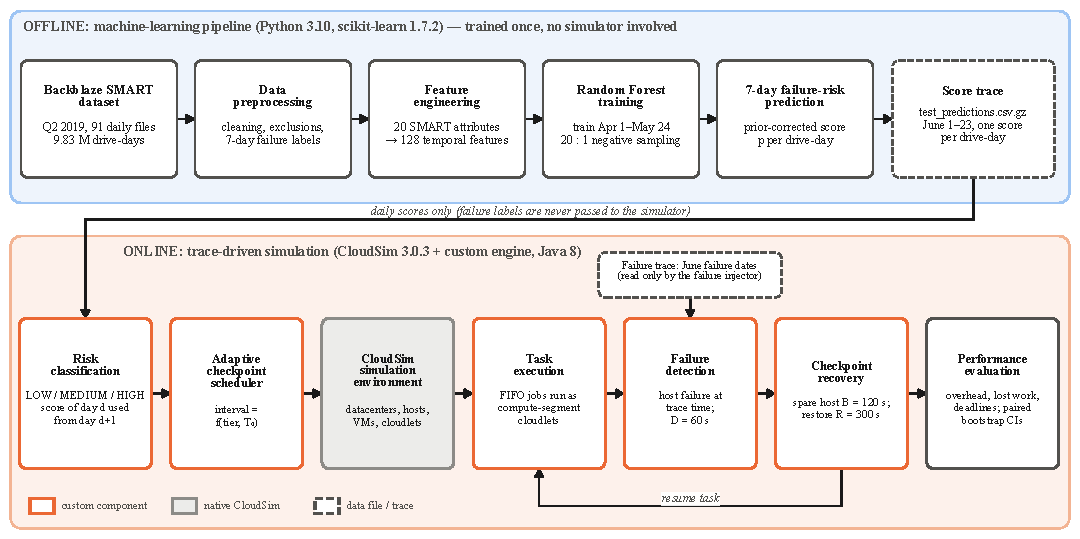
\includegraphics[width=\textwidth]{figures/fig01_system_architecture.pdf}
  \caption{\CapFigZeroOneSystemArchitecture}
  \label{fig:system_architecture}
\end{figure*}

\begin{figure}[!t]
  \centering
  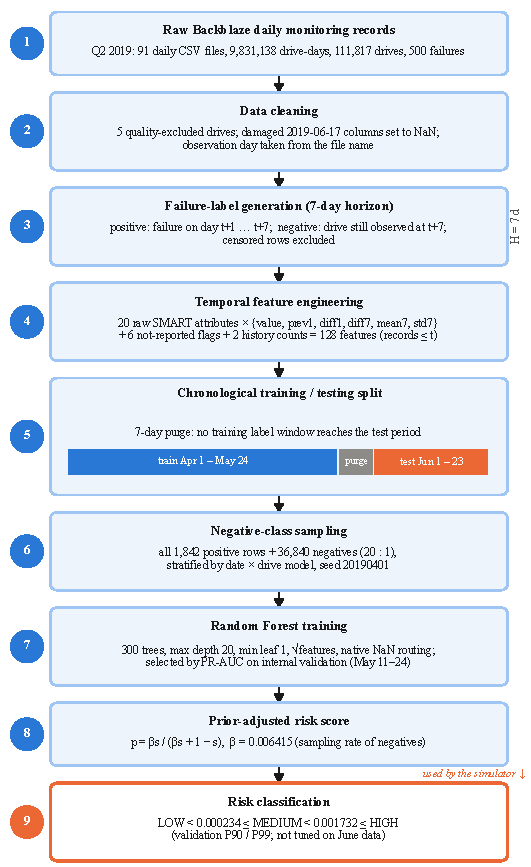
\includegraphics[width=\columnwidth]{figures/fig02_ml_pipeline.pdf}
  \caption{\CapFigZeroTwoMlPipeline}
  \label{fig:ml_pipeline}
\end{figure}

\begin{figure}[!t]
  \centering
  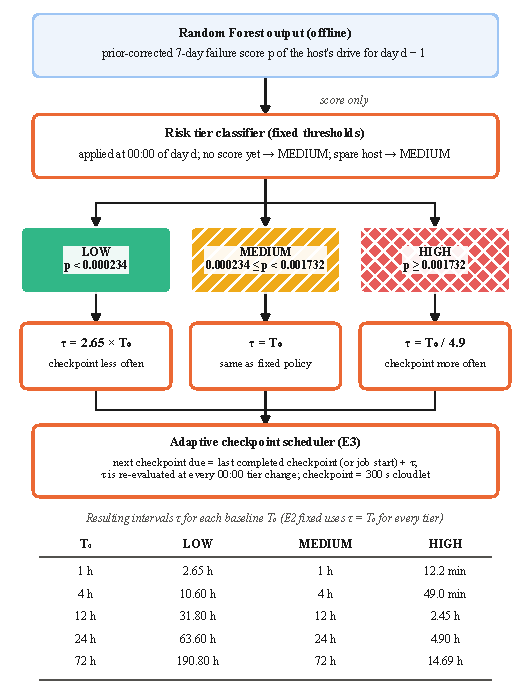
\includegraphics[width=\columnwidth]{figures/fig03_adaptive_checkpointing.pdf}
  \caption{\CapFigZeroThreeAdaptiveCheckpointing}
  \label{fig:adaptive}
\end{figure}

\begin{figure*}[!t]
  \centering
  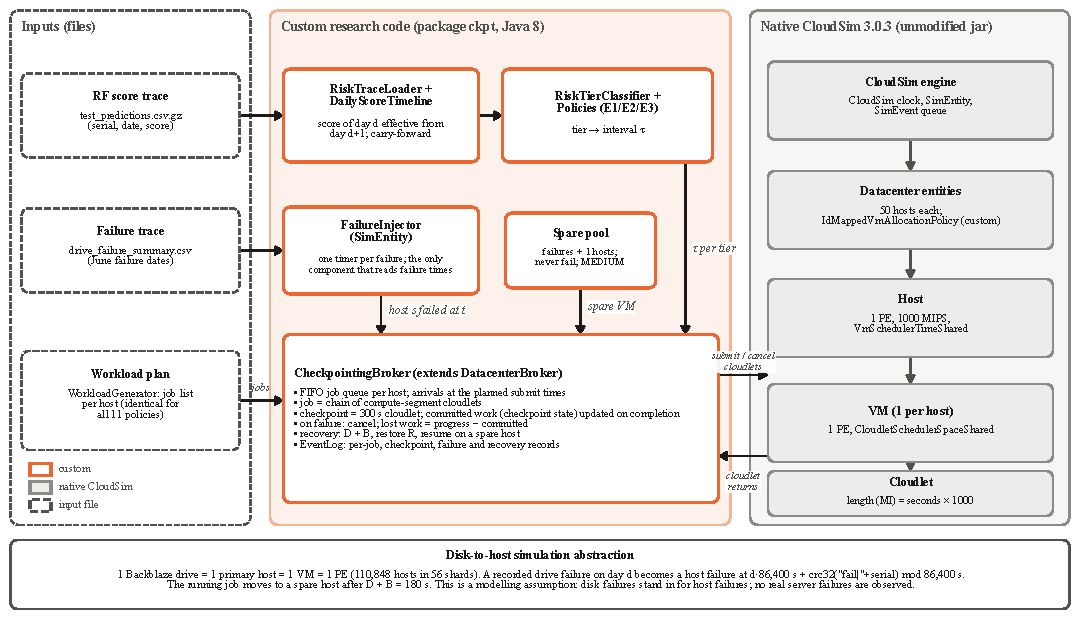
\includegraphics[width=\textwidth]{figures/fig04_cloudsim_integration.pdf}
  \caption{\CapFigZeroFourCloudsimIntegration}
  \label{fig:cloudsim}
\end{figure*}

\begin{figure*}[!t]
  \centering
  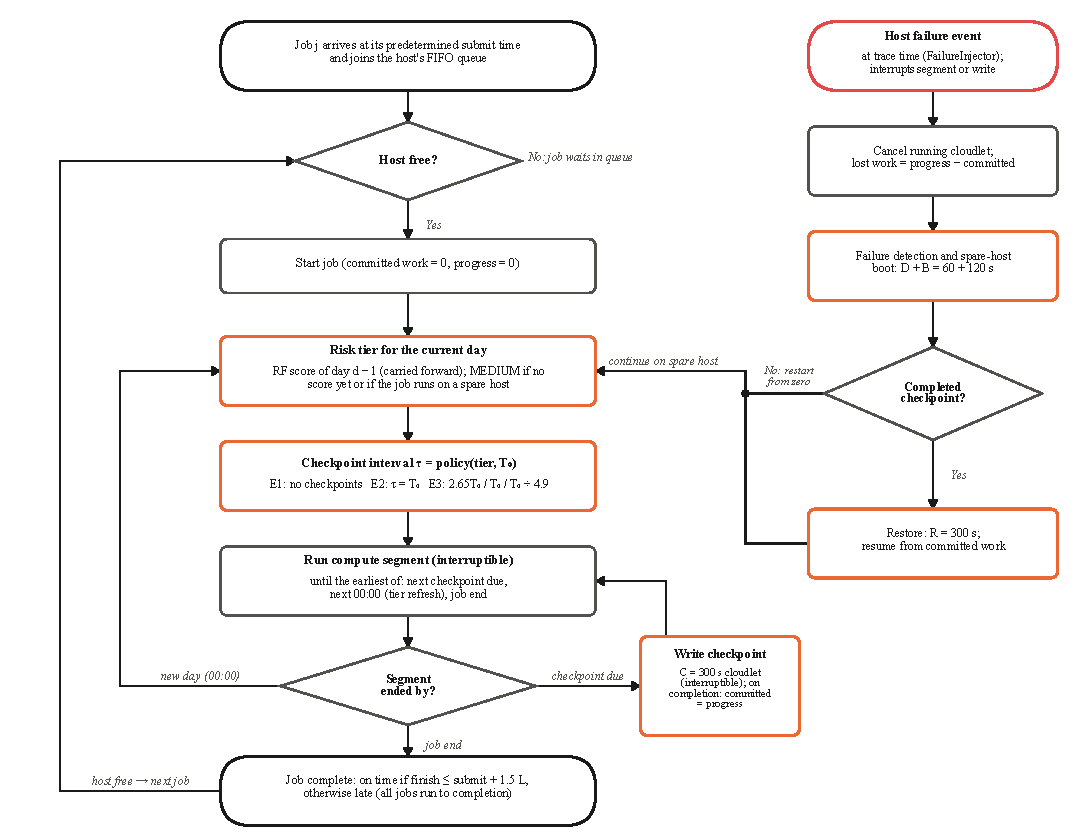
\includegraphics[width=\textwidth]{figures/fig05_execution_flow.pdf}
  \caption{\CapFigZeroFiveExecutionFlow}
  \label{fig:execution_flow}
\end{figure*}

\begin{figure*}[!t]
  \centering
  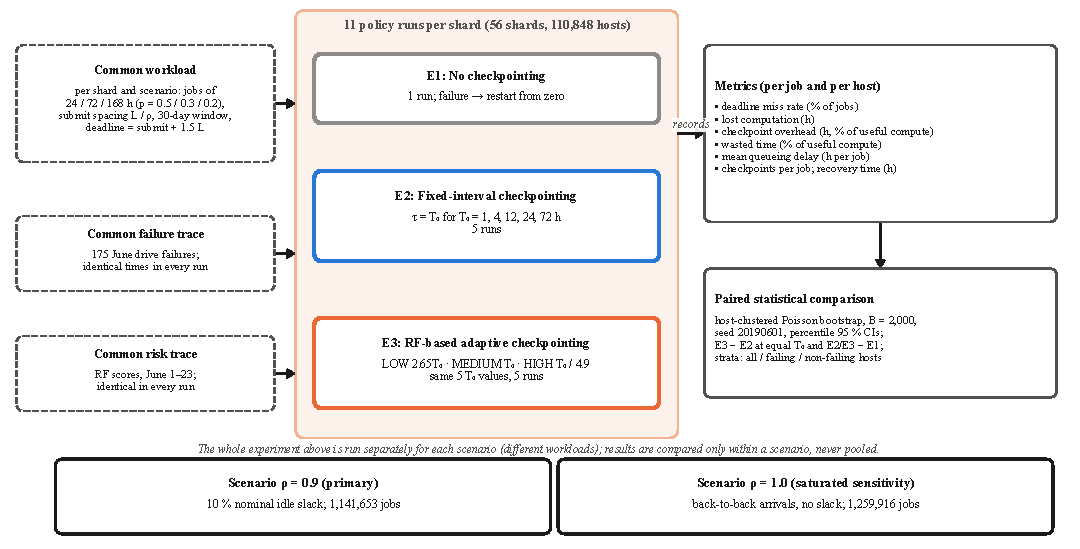
\includegraphics[width=\textwidth]{figures/fig06_experimental_design.pdf}
  \caption{\CapFigZeroSixExperimentalDesign}
  \label{fig:experimental_design}
\end{figure*}

\begin{figure}[!t]
  \centering
  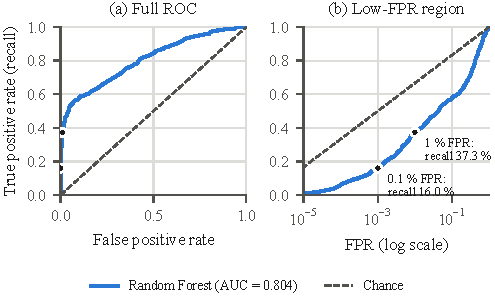
\includegraphics[width=\columnwidth]{figures/g01_rf_roc_curve.pdf}
  \caption{\CapGZeroOneRfRocCurve}
  \label{fig:rf_roc}
\end{figure}

\begin{figure}[!t]
  \centering
  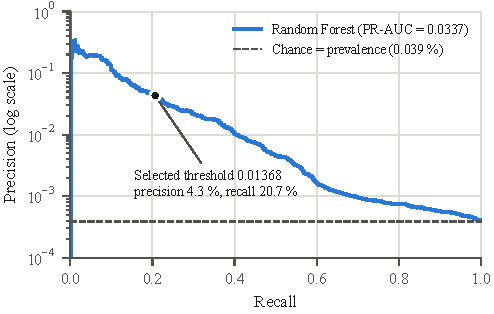
\includegraphics[width=\columnwidth]{figures/g02_rf_precision_recall_curve.pdf}
  \caption{\CapGZeroTwoRfPrecisionRecallCurve}
  \label{fig:rf_pr}
\end{figure}

\begin{figure*}[!t]
  \centering
  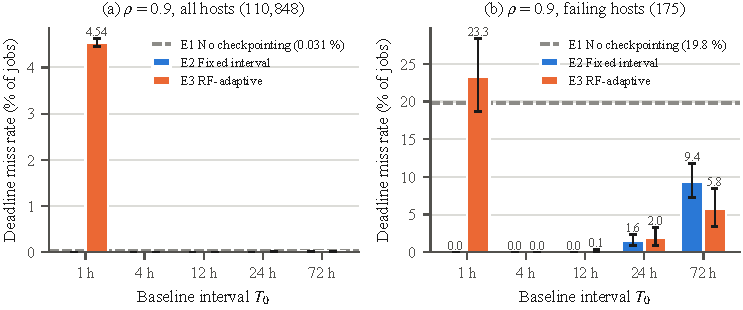
\includegraphics[width=0.75\textwidth]{figures/g08_deadline_miss_vs_T0_rho09.pdf}
  \caption{\CapGZeroEightDeadlineMissVsTZeroRhoZeroNine}
  \label{fig:deadline_rho09}
\end{figure*}

\begin{figure}[!t]
  \centering
  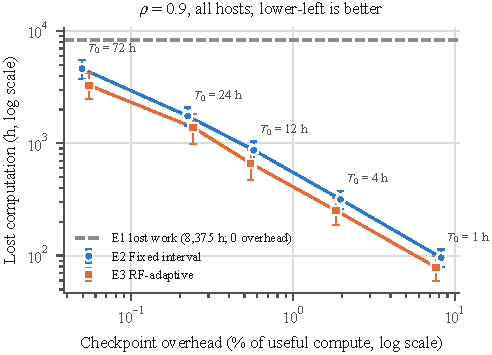
\includegraphics[width=\columnwidth]{figures/g10_overhead_vs_lost_tradeoff_rho09.pdf}
  \caption{\CapGTenOverheadVsLostTradeoffRhoZeroNine}
  \label{fig:tradeoff_rho09}
\end{figure}

\begin{figure*}[!t]
  \centering
  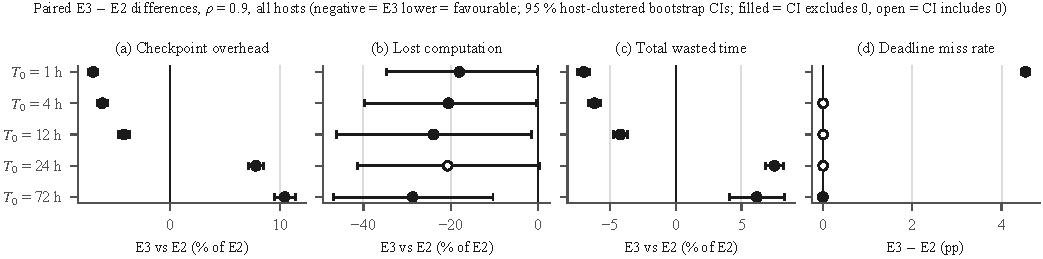
\includegraphics[width=\textwidth]{figures/g12_paired_E3_vs_E2_rho09.pdf}
  \caption{\CapGTwelvePairedEThreeVsETwoRhoZeroNine}
  \label{fig:paired_rho09}
\end{figure*}

\begin{figure*}[!t]
  \centering
  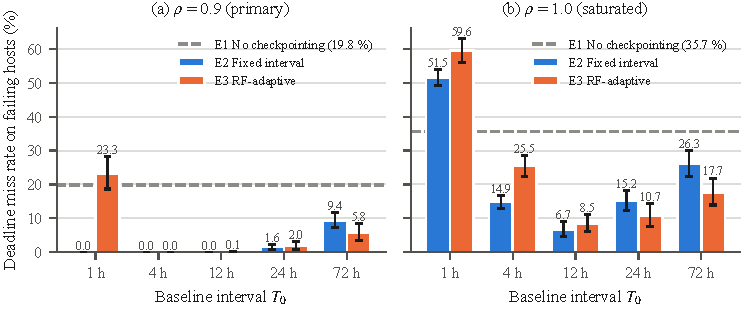
\includegraphics[width=0.75\textwidth]{figures/g16_failing_host_deadline_miss_both_rho.pdf}
  \caption{\CapGSixteenFailingHostDeadlineMissBothRho}
  \label{fig:failing_deadline}
\end{figure*}

\begin{figure}[!t]
  \centering
  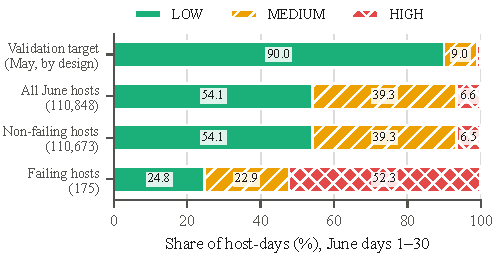
\includegraphics[width=\columnwidth]{figures/g17_tier_occupancy.pdf}
  \caption{\CapGSeventeenTierOccupancy}
  \label{fig:tier_occupancy}
\end{figure}

\begin{figure*}[!t]
  \centering
  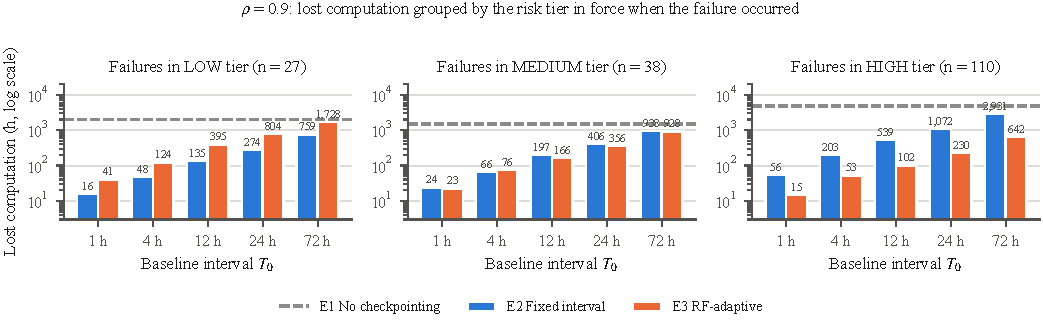
\includegraphics[width=\textwidth]{figures/g19_lost_work_by_tier_rho09.pdf}
  \caption{\CapGNineteenLostWorkByTierRhoZeroNine}
  \label{fig:lost_tier_rho09}
\end{figure*}

% Auto-generated by paper_assets/scripts/make_tables.py from project/ml/results/dataset_audit_revalidation/dataset_summary.txt, project/ml/processed/feature_manifest.md
\begin{table}[!t]
\centering
\caption{Backblaze Q2 2019 dataset characteristics.}
\label{tab:dataset}
\footnotesize
\setlength{\tabcolsep}{4pt}
\begin{tabular}{lp{0.58\columnwidth}}
\toprule
Characteristic & Value \\
\midrule
Source & Backblaze hard-drive statistics, Q2 2019 (daily SMART snapshots) \\
Observation period & 2019-04-01 to 2019-06-30 \\
Daily files & 91 / 91 \\
Drive-day records & 9,831,138 \\
Unique drives (serial numbers) & 111,817 \\
Drive models & 42 \\
Failure records (= failed drives) & 500 \\
Row-level failure rate & 0.0051 \%  (1 : 19,662) \\
Annualised failure rate & 1.86 \\
Daily drive count (min / median / max) & 105,624 / 108,216 / 110,718 \\
Columns & 129  (5 identifier columns + 124 SMART columns) \\
SMART raw attributes used & 20 (14 core, $\le$5 \% missing; 6 partial: 187, 188, 190, 240, 241, 242) \\
Known file anomaly & 2019-06-17.csv spreadsheet-altered (CR-only, non-ISO dates, scientific notation); damaged columns set to NaN \\
\bottomrule
\end{tabular}
\end{table}

% Auto-generated by paper_assets/scripts/make_tables.py from project/ml/results/model_evaluation/validation_metrics.json, project/ml/results/model_evaluation/test_metrics.json
\begin{table}[!t]
\centering
\caption{Random Forest predictive performance (7-day horizon).}
\label{tab:rf_performance}
\footnotesize
\setlength{\tabcolsep}{4pt}
\begin{tabular}{lrr}
\toprule
Metric & Validation & Test (June) \\
\midrule
Drive-day rows & 1,508,766 & 2,544,754 \\
Positive rows & 481 & 997 \\
Prevalence (\%) & 0.032 & 0.039 \\
PR-AUC & 0.0485 & 0.0337 \\
ROC-AUC & 0.853 & 0.804 \\
Recall at 0.1 \% FPR (\%) & 27.2 & 16.0 \\
Recall at 1 \% FPR (\%) & 52.4 & 37.3 \\
Brier score & 0.000313 & 0.000387 \\
Brier, constant-prevalence reference & 0.000319 & 0.000392 \\
Precision at threshold (\%) & 9.5 & 4.3 \\
Recall at threshold (\%) & 23.5 & 20.7 \\
FPR at threshold (\%) & 0.071 & 0.181 \\
TP / FP / FN & 113 / 1,078 / 368 & 206 / 4,597 / 791 \\
\midrule
Failed drives in period & 107 & 175 \\
Failed drives with $\ge$1 alarm (\%) & 34.6 & 33.7 \\
Median lead time (days) & 4 & 4 \\
False alarms per 1,000 drive-days & 0.71 & 1.81 \\
Healthy drives with $\ge$1 alarm (\%) & 0.17 & 1.48 \\
\bottomrule
\end{tabular}
\par\smallskip
\parbox{0.97\columnwidth}{\scriptsize Validation: 2019-05-11 -- 05-24 (internal-validation model, used to choose hyper-parameters and the threshold 0.01368). Test: June 1 -- 23, evaluated once with the final model. Row level: each drive-day is one prediction. Drive level: a failed drive counts as detected if it has at least one alarm in its 7-day pre-failure window. A random ranking has PR-AUC equal to the prevalence.}
\end{table}

% Auto-generated by paper_assets/scripts/make_tables.py from project/cloudsim/research/src/ckpt/policy/RiskTierClassifier.java, project/cloudsim/research/src/ckpt/policy/Policies.java, project/cloudsim/results/full_rho0.9/analysis/tier_occupancy.csv
\begin{table*}[!t]
\centering
\caption{Risk tiers and adaptive checkpoint-interval rules (E3).}
\label{tab:tiers}
\footnotesize
\setlength{\tabcolsep}{4pt}
\begin{tabular}{lllrrrrrrr}
\toprule
\multicolumn{3}{c}{} & \multicolumn{5}{c}{E3 interval $\tau$ at baseline $T_0$} & \multicolumn{2}{c}{Host-day share} \\
\cmidrule(lr){4-8} \cmidrule(lr){9-10}
Tier & Score range & E3 rule & $T_0$=1h & $T_0$=4h & $T_0$=12h & $T_0$=24h & $T_0$=72h & Design \% & June \% \\
\midrule
LOW & p $<$ 0.000234 & 2.65 $\times$ $T_0$ & 2.6 h & 10.6 h & 31.8 h & 63.6 h & 190.8 h & 90 & 54.1 \\
MEDIUM & 0.000234 $\le$ p $<$ 0.001732 & $T_0$ & 1.0 h & 4.0 h & 12.0 h & 24.0 h & 72.0 h & 9 & 39.3 \\
HIGH & p $\ge$ 0.001732 & $T_0$ / 4.9 & 12 min & 49 min & 2.4 h & 4.9 h & 14.7 h & 1 & 6.6 \\
\bottomrule
\end{tabular}
\par\smallskip
\parbox{0.97\textwidth}{\scriptsize p is the prior-corrected 7-day failure score. Boundaries are the P90 (0.000234) and P99 (0.001732) of internal-validation scores (May 11 -- 24) and were not tuned on June data. The score of day d sets the tier from 00:00 of day d+1 (carried forward if missing; MEDIUM before any score and on spare hosts). E2 uses $\tau$ = $T_0$ for every tier; E1 never checkpoints. Design share = intended share on validation; June share = observed share of host-days.}
\end{table*}

% Auto-generated by paper_assets/scripts/make_tables.py from project/cloudsim/research/src/ckpt/sim/SimParams.java, project/cloudsim/results/full_rho0.9/run_config.json, project/cloudsim/research/src/ckpt/sim/SimulationRunner.java, project/cloudsim/research/src/ckpt/ExperimentRunner.java
\begin{table}[!t]
\centering
\caption{CloudSim simulation configuration.}
\label{tab:cloudsim_config}
\footnotesize
\setlength{\tabcolsep}{4pt}
\begin{tabular}{lp{0.58\columnwidth}}
\toprule
Item & Value \\
\midrule
Simulator & CloudSim 3.0.3 (official jar, unmodified) + custom package ckpt \\
Runtime & compiled with javac --release 8; run on Java 1.8.0\_501 \\
Hosts (= drives) & 110,848 in 56 shards, crc32(serial) mod 56 \\
Host / VM & 1 PE at 1000 MIPS; 1 VM per host, space-shared cloudlet scheduler \\
Datacenter entities & 50 hosts each (performance grouping only) \\
Checkpoint save time C & 300 s \\
Restore time R & 300 s \\
Failure detection D & 60 s \\
Replacement boot B & 120 s \\
Deadline & submit + 1.5 $\times$ job length \\
Spare hosts per shard & failures in shard + 1; never fail; MEDIUM tier \\
Failure time & day d + crc32("fail$|$"+serial) mod 86,400 s \\
Recovery without checkpoint & restart from zero after D + B (no R) \\
Segment rule & compute segment ends at earliest of: checkpoint due, 00:00, job end \\
Policies $\times$ baselines & E1; E2 and E3 at $T_0$ = 1, 4, 12, 24, 72 h (11 runs per shard) \\
\bottomrule
\end{tabular}
\end{table}

% Auto-generated by paper_assets/scripts/make_tables.py from project/cloudsim/research/src/ckpt/trace/WorkloadGenerator.java, project/cloudsim/results/full_rho0.9/analysis/analysis_meta.json, project/cloudsim/results/full_rho1.0/analysis/analysis_meta.json
\begin{table*}[!t]
\centering
\caption{Workload model and experimental scenarios.}
\label{tab:workload}
\footnotesize
\setlength{\tabcolsep}{4pt}
\begin{tabular}{lp{0.50\textwidth}r}
\toprule
Item & Definition & Count \\
\midrule
Job lengths L & 24 h / 72 h / 168 h with p = 0.5 / 0.3 / 0.2 (crc32(serial$|$j) mod 10) &  \\
Arrivals & submit(j+1) = submit(j) + L(j) / $\rho$ from the host's first day; FIFO queue per host &  \\
Generation window & jobs generated while submit $<$ 30 days; all jobs run to completion &  \\
Deadline & submit + 1.5 L (late jobs counted, never dropped) &  \\
Identical across policies & job ids, lengths, submit times, failure trace, risk trace &  \\
Scenario $\rho$ = 0.9 (primary) & 10 \% nominal idle slack & 1,141,653 jobs \\
Scenario $\rho$ = 1.0 (sensitivity) & back-to-back nominal arrivals, no slack & 1,259,916 jobs \\
Hosts / failing hosts & same in both scenarios & 110,848 / 175 \\
\bottomrule
\end{tabular}
\par\smallskip
\parbox{0.97\textwidth}{\scriptsize Job counts differ between scenarios because $\rho$ changes the submit spacing; raw totals are therefore not compared across scenarios.}
\end{table*}

% Auto-generated by paper_assets/scripts/make_tables.py from project/cloudsim/results/full_rho0.9/analysis/policy_summary.csv
\begin{table*}[!t]
\centering
\caption{Overall policy comparison, $\rho$ = 0.9 (primary).}
\label{tab:policy_rho09}
\footnotesize
\setlength{\tabcolsep}{4pt}
\begin{tabular}{lrrrrrrrrr}
\toprule
Policy & Miss \% & Lost (h) & Lost 95 \% CI & Overhead (h) & Ovh. \% & Waste \% & Queue h/job & Ckpt/job & Recov. (h) \\
\midrule
E1 none & 0.031 & 8,375 & [6,703, 10,108] & 0 & 0 & 0.011 & 0.019 & 0 & 7.75 \\
\midrule
E2 fixed, $T_0$ = 1 h & 0 & 96.02 & [79.36, 113.3] & 6,293,612 & 8.21 & 8.21 & 5.5e-06 & 66.15 & 22.82 \\
E3 adaptive, $T_0$ = 1 h & 4.54 & 78.72 & [59.42, 99.26] & 5,852,951 & 7.63 & 7.63 & 2.30 & 61.52 & 22.98 \\
\midrule
E2 fixed, $T_0$ = 4 h & 0 & 317.8 & [261.0, 375.7] & 1,502,050 & 1.96 & 1.96 & 1.4e-05 & 15.79 & 20.18 \\
E3 adaptive, $T_0$ = 4 h & 0 & 252.5 & [188.4, 325.0] & 1,409,313 & 1.84 & 1.84 & 1.2e-05 & 14.81 & 21.28 \\
\midrule
E2 fixed, $T_0$ = 12 h & 0 & 871.3 & [706.6, 1,037] & 437,258 & 0.570 & 0.572 & 0.0001 & 4.60 & 18.85 \\
E3 adaptive, $T_0$ = 12 h & 0.0002 & 662.8 & [473.0, 868.8] & 419,017 & 0.547 & 0.547 & 0.0002 & 4.40 & 19.00 \\
\midrule
E2 fixed, $T_0$ = 24 h & 0.0025 & 1,753 & [1,442, 2,082] & 171,060 & 0.223 & 0.225 & 0.0008 & 1.80 & 16.58 \\
E3 adaptive, $T_0$ = 24 h & 0.0031 & 1,390 & [988.0, 1,813] & 184,379 & 0.240 & 0.242 & 0.0014 & 1.94 & 18.00 \\
\midrule
E2 fixed, $T_0$ = 72 h & 0.015 & 4,627 & [3,742, 5,565] & 37,985 & 0.050 & 0.056 & 0.0063 & 0.399 & 11.17 \\
E3 adaptive, $T_0$ = 72 h & 0.0091 & 3,298 & [2,476, 4,214] & 41,935 & 0.055 & 0.059 & 0.0056 & 0.441 & 15.50 \\
\bottomrule
\end{tabular}
\par\smallskip
\parbox{0.97\textwidth}{\scriptsize $\rho$ = 0.9, all 110,848 hosts, 1,141,653 jobs, 175 failures. Miss \% = late jobs / jobs. Lost = computation lost to failures. Overhead = 300 s $\times$ completed checkpoint writes (writes cut short by a failure are counted in Waste). Ovh. \% and Waste \% are percentages of useful compute (sum of job lengths); Waste = overhead + lost + interrupted writes + recovery. Queue = mean waiting time before a job starts. Lost-work CIs: paired host-clustered bootstrap (B = 2,000).}
\end{table*}

% Auto-generated by paper_assets/scripts/make_tables.py from project/cloudsim/results/full_rho0.9/analysis/paired_comparisons.csv
\begin{table*}[!t]
\centering
\caption{Paired E3 $-$ E2 comparison at equal $T_0$, $\rho$ = 0.9, all hosts.}
\label{tab:paired_rho09}
\footnotesize
\setlength{\tabcolsep}{4pt}
\begin{tabular}{llrrrrrl}
\toprule
$T_0$ & Metric & E2 & E3 & $\Delta$ & $\Delta$ \% & 95 \% CI of $\Delta$ & Assessment \\
\midrule
1 h & Overhead (h) & 6,293,612 & 5,852,951 & $-$440,661 & $-$7.0 & [$-$467,886, $-$412,600] & E3 lower (favourable) \\
 & Lost work (h) & 96.02 & 78.72 & $-$17.31 & $-$18.0 & [$-$33.41, $-$0.058] & E3 lower (favourable) \\
 & Wasted (\% useful) & 8.21 & 7.63 & $-$0.575 & $-$7.0 & [$-$0.611, $-$0.539] & E3 lower (favourable) \\
 & Deadline miss (\%) & 0 & 4.54 & +4.54 & -- & [4.45, 4.62] & E3 higher (unfavourable) \\
 & Queue (h/job) & 5.5e-06 & 2.30 & +2.30 & -- & [2.25, 2.35] & E3 higher (unfavourable) \\
\midrule
4 h & Overhead (h) & 1,502,050 & 1,409,313 & $-$92,736 & $-$6.2 & [$-$99,504, $-$85,803] & E3 lower (favourable) \\
 & Lost work (h) & 317.8 & 252.5 & $-$65.26 & $-$20.5 & [$-$126.4, $-$1.34] & E3 lower (favourable) \\
 & Wasted (\% useful) & 1.96 & 1.84 & $-$0.121 & $-$6.2 & [$-$0.130, $-$0.112] & E3 lower (favourable) \\
 & Deadline miss (\%) & 0 & 0 & 0 & -- & [0, 0] & no difference \\
 & Queue (h/job) & 1.4e-05 & 1.2e-05 & $-$1.9e-06 & -- & [$-$1.1e-05, 8.2e-06] & inconclusive (CI incl. 0) \\
\midrule
12 h & Overhead (h) & 437,258 & 419,017 & $-$18,241 & $-$4.2 & [$-$20,459, $-$15,976] & E3 lower (favourable) \\
 & Lost work (h) & 871.3 & 662.8 & $-$208.5 & $-$23.9 & [$-$402.1, $-$12.87] & E3 lower (favourable) \\
 & Wasted (\% useful) & 0.572 & 0.547 & $-$0.024 & $-$4.2 & [$-$0.027, $-$0.021] & E3 lower (favourable) \\
 & Deadline miss (\%) & 0 & 0.0002 & +0.0002 & -- & [0, 0.0004] & inconclusive (CI incl. 0) \\
 & Queue (h/job) & 0.0001 & 0.0002 & +6.6e-05 & -- & [$-$6.3e-05, 0.0002] & inconclusive (CI incl. 0) \\
\midrule
24 h & Overhead (h) & 171,060 & 184,379 & +13,319 & +7.8 & [12,226, 14,446] & E3 higher (unfavourable) \\
 & Lost work (h) & 1,753 & 1,390 & $-$362.6 & $-$20.7 & [$-$726.5, 7.22] & inconclusive (CI incl. 0) \\
 & Wasted (\% useful) & 0.225 & 0.242 & +0.017 & +7.5 & [0.015, 0.018] & E3 higher (unfavourable) \\
 & Deadline miss (\%) & 0.0025 & 0.0031 & +0.0006 & -- & [$-$0.0015, 0.0028] & inconclusive (CI incl. 0) \\
 & Queue (h/job) & 0.0008 & 0.0014 & +0.0006 & -- & [$-$7.7e-05, 0.0014] & inconclusive (CI incl. 0) \\
\midrule
72 h & Overhead (h) & 37,985 & 41,935 & +3,950 & +10.4 & [3,596, 4,313] & E3 higher (unfavourable) \\
 & Lost work (h) & 4,627 & 3,298 & $-$1,329 & $-$28.7 & [$-$2,172, $-$477.8] & E3 lower (favourable) \\
 & Wasted (\% useful) & 0.056 & 0.059 & +0.0034 & +6.2 & [0.0023, 0.0046] & E3 higher (unfavourable) \\
 & Deadline miss (\%) & 0.015 & 0.0091 & $-$0.0056 & -- & [$-$0.011, $-$0.0004] & E3 lower (favourable) \\
 & Queue (h/job) & 0.0063 & 0.0056 & $-$0.0006 & -- & [$-$0.0032, 0.0024] & inconclusive (CI incl. 0) \\
\bottomrule
\end{tabular}
\par\smallskip
\parbox{0.97\textwidth}{\scriptsize Paired within $\rho$ = 0.9: E2 and E3 at the same $T_0$ run the identical workload, failures and risk trace. $\Delta$ = E3 $-$ E2; lower is favourable for every metric. $\Delta$ \% = $\Delta$ / E2 (given only for totals; deadline and queue differences are absolute, in percentage points or h/job). 95 \% CI: paired host-clustered Poisson bootstrap (B = 2,000, seed 20190601) on the difference; shards are not treated as samples. Intervals are not adjusted for multiple comparisons and are descriptive only; no significance is claimed. Lost-work intervals rest on 175 failure events and are wide.}
\end{table*}

% Auto-generated by paper_assets/scripts/make_tables.py from project/cloudsim/results/full_rho1.0/analysis/paired_comparisons.csv
\begin{table*}[!t]
\centering
\caption{Paired E3 $-$ E2 comparison at equal $T_0$, $\rho$ = 1.0, all hosts.}
\label{tab:paired_rho10}
\footnotesize
\setlength{\tabcolsep}{4pt}
\begin{tabular}{llrrrrrl}
\toprule
$T_0$ & Metric & E2 & E3 & $\Delta$ & $\Delta$ \% & 95 \% CI of $\Delta$ & Assessment \\
\midrule
1 h & Overhead (h) & 6,945,035 & 6,554,774 & $-$390,261 & $-$5.6 & [$-$420,480, $-$358,967] & E3 lower (favourable) \\
 & Lost work (h) & 96.77 & 78.68 & $-$18.09 & $-$18.7 & [$-$35.79, 0.297] & inconclusive (CI incl. 0) \\
 & Wasted (\% useful) & 8.21 & 7.75 & $-$0.461 & $-$5.6 & [$-$0.497, $-$0.425] & E3 lower (favourable) \\
 & Deadline miss (\%) & 50.74 & 34.23 & $-$16.51 & -- & [$-$16.61, $-$16.41] & E3 lower (favourable) \\
 & Queue (h/job) & 26.83 & 19.06 & $-$7.77 & -- & [$-$7.86, $-$7.69] & E3 lower (favourable) \\
\midrule
4 h & Overhead (h) & 1,657,514 & 1,559,670 & $-$97,844 & $-$5.9 & [$-$105,265, $-$90,212] & E3 lower (favourable) \\
 & Lost work (h) & 354.0 & 278.7 & $-$75.23 & $-$21.3 & [$-$138.4, $-$6.20] & E3 lower (favourable) \\
 & Wasted (\% useful) & 1.96 & 1.84 & $-$0.116 & $-$5.9 & [$-$0.124, $-$0.107] & E3 lower (favourable) \\
 & Deadline miss (\%) & 7.64 & 3.23 & $-$4.41 & -- & [$-$4.48, $-$4.33] & E3 lower (favourable) \\
 & Queue (h/job) & 6.37 & 4.44 & $-$1.93 & -- & [$-$1.95, $-$1.91] & E3 lower (favourable) \\
\midrule
12 h & Overhead (h) & 482,509 & 462,438 & $-$20,071 & $-$4.2 & [$-$22,505, $-$17,547] & E3 lower (favourable) \\
 & Lost work (h) & 1,058 & 726.5 & $-$331.5 & $-$31.3 & [$-$525.0, $-$143.7] & E3 lower (favourable) \\
 & Wasted (\% useful) & 0.572 & 0.548 & $-$0.024 & $-$4.2 & [$-$0.027, $-$0.021] & E3 lower (favourable) \\
 & Deadline miss (\%) & 0.011 & 0.265 & +0.254 & -- & [0.237, 0.271] & E3 higher (unfavourable) \\
 & Queue (h/job) & 1.82 & 1.24 & $-$0.584 & -- & [$-$0.591, $-$0.577] & E3 lower (favourable) \\
\midrule
24 h & Overhead (h) & 188,758 & 200,507 & +11,749 & +6.2 & [10,564, 12,958] & E3 higher (unfavourable) \\
 & Lost work (h) & 2,031 & 1,671 & $-$360.7 & $-$17.8 & [$-$769.3, 43.23] & inconclusive (CI incl. 0) \\
 & Wasted (\% useful) & 0.226 & 0.239 & +0.013 & +6.0 & [0.012, 0.015] & E3 higher (unfavourable) \\
 & Deadline miss (\%) & 0.024 & 0.017 & $-$0.0071 & -- & [$-$0.014, $-$0.0008] & E3 lower (favourable) \\
 & Queue (h/job) & 0.688 & 0.522 & $-$0.166 & -- & [$-$0.170, $-$0.162] & E3 lower (favourable) \\
\midrule
72 h & Overhead (h) & 41,917 & 43,586 & +1,669 & +4.0 & [1,298, 2,067] & E3 higher (unfavourable) \\
 & Lost work (h) & 5,136 & 3,687 & $-$1,449 & $-$28.2 & [$-$2,300, $-$571.1] & E3 lower (favourable) \\
 & Wasted (\% useful) & 0.056 & 0.056 & +0.0003 & +0.5 & [$-$0.0008, 0.0014] & inconclusive (CI incl. 0) \\
 & Deadline miss (\%) & 0.042 & 0.028 & $-$0.014 & -- & [$-$0.021, $-$0.0068] & E3 lower (favourable) \\
 & Queue (h/job) & 0.158 & 0.098 & $-$0.061 & -- & [$-$0.065, $-$0.056] & E3 lower (favourable) \\
\bottomrule
\end{tabular}
\par\smallskip
\parbox{0.97\textwidth}{\scriptsize Paired within $\rho$ = 1.0: E2 and E3 at the same $T_0$ run the identical workload, failures and risk trace. $\Delta$ = E3 $-$ E2; lower is favourable for every metric. $\Delta$ \% = $\Delta$ / E2 (given only for totals; deadline and queue differences are absolute, in percentage points or h/job). 95 \% CI: paired host-clustered Poisson bootstrap (B = 2,000, seed 20190601) on the difference; shards are not treated as samples. Intervals are not adjusted for multiple comparisons and are descriptive only; no significance is claimed. Lost-work intervals rest on 175 failure events and are wide.}
\end{table*}

% Auto-generated by paper_assets/scripts/make_tables.py from project/cloudsim/results/full_rho0.9/analysis/policy_summary.csv
\begin{table*}[!t]
\centering
\caption{Failing versus non-failing hosts, $\rho$ = 0.9.}
\label{tab:strata_rho09}
\footnotesize
\setlength{\tabcolsep}{4pt}
\begin{tabular}{lrrrrrrrrr}
\toprule
 & \multicolumn{5}{c}{Failing hosts (175)} & \multicolumn{4}{c}{Non-failing hosts (110,673)} \\
\cmidrule(lr){2-6} \cmidrule(lr){7-10}
Policy & Miss \% & 95 \% CI & Lost (h) & Ovh. \% & Ckpt/job & Miss \% & Ovh. \% & Ckpt/job & Queue h/job \\
\midrule
E1 none & 19.81 & [15.98, 24.07] & 8,375 & 0 & 0 & 0 & 0 & 0 & 2.7e-06 \\
\midrule
E2 fixed, $T_0$ = 1 h & 0 & [0, 0] & 96.02 & 8.21 & 66.25 & 0 & 8.21 & 66.15 & 2.7e-06 \\
E3 adaptive, $T_0$ = 1 h & 23.34 & [18.66, 28.35] & 78.72 & 11.94 & 96.35 & 4.51 & 7.63 & 61.47 & 2.28 \\
\midrule
E2 fixed, $T_0$ = 4 h & 0 & [0, 0] & 317.8 & 1.96 & 15.81 & 0 & 1.96 & 15.79 & 2.7e-06 \\
E3 adaptive, $T_0$ = 4 h & 0 & [0, 0] & 252.5 & 3.18 & 25.64 & 0 & 1.84 & 14.80 & 2.7e-06 \\
\midrule
E2 fixed, $T_0$ = 12 h & 0 & [0, 0] & 871.3 & 0.571 & 4.60 & 0 & 0.570 & 4.60 & 2.7e-06 \\
E3 adaptive, $T_0$ = 12 h & 0.112 & [0, 0.299] & 662.8 & 0.988 & 7.97 & 0 & 0.546 & 4.40 & 2.7e-06 \\
\midrule
E2 fixed, $T_0$ = 24 h & 1.57 & [0.843, 2.37] & 1,753 & 0.223 & 1.80 & 0 & 0.223 & 1.80 & 2.7e-06 \\
E3 adaptive, $T_0$ = 24 h & 1.96 & [0.896, 3.24] & 1,390 & 0.441 & 3.56 & 0 & 0.240 & 1.94 & 2.7e-06 \\
\midrule
E2 fixed, $T_0$ = 72 h & 9.40 & [7.23, 11.74] & 4,627 & 0.050 & 0.406 & 0 & 0.050 & 0.399 & 2.7e-06 \\
E3 adaptive, $T_0$ = 72 h & 5.82 & [3.47, 8.49] & 3,298 & 0.121 & 0.980 & 0 & 0.055 & 0.440 & 2.7e-06 \\
\bottomrule
\end{tabular}
\par\smallskip
\parbox{0.97\textwidth}{\scriptsize $\rho$ = 0.9. Failing hosts: the 175 hosts whose drive failed in June (one failure each); non-failing: 110,673 hosts. Non-failing hosts lose no work by construction. CI: host-clustered bootstrap within the stratum.}
\end{table*}

% Auto-generated by paper_assets/scripts/make_tables.py from project/cloudsim/results/full_rho0.9/analysis/tier_occupancy.csv, project/cloudsim/results/full_rho0.9/analysis/analysis_meta.json, project/cloudsim/results/full_rho0.9/analysis/failures_detail.csv
\begin{table*}[!t]
\centering
\caption{Risk-tier occupancy and failure distribution (June 2019).}
\label{tab:tier_occupancy}
\footnotesize
\setlength{\tabcolsep}{4pt}
\begin{tabular}{lrrrrr}
\toprule
Group & Hosts & Host-days & LOW & MEDIUM & HIGH \\
\midrule
All hosts & 110,848 & 3,325,440 & 54.09 & 39.30 & 6.61 \\
Failing hosts & 175 & 5,250 & 24.78 & 22.91 & 52.30 \\
Non-failing hosts & 110,673 & 3,320,190 & 54.14 & 39.33 & 6.53 \\
Validation design target & -- & -- & 90.00 & 9.00 & 1.00 \\
\midrule
Hosts by majority June tier & 110,848 & -- & 92,493 & 15,675 & 2,680 \\
Failing hosts by majority tier & 175 & -- & 42 & 37 & 96 \\
Failures by tier at failure instant & 175 & -- & 27 (15.4 \%) & 38 (21.7 \%) & 110 (62.9 \%) \\
\bottomrule
\end{tabular}
\par\smallskip
\parbox{0.97\textwidth}{\scriptsize Host-day shares cover June days 1 -- 30 and are identical in both scenarios (the risk trace does not depend on $\rho$). The design target is the share implied by the P90 / P99 validation boundaries. Failures by tier are identical in all 11 policies and both $\rho$ values.}
\end{table*}

% Auto-generated by paper_assets/scripts/make_tables.py from project/cloudsim/results/full_rho0.9/validation/validation_summary.json, project/cloudsim/results/full_rho1.0/validation/validation_summary.json, project/cloudsim/results/full_rho0.9/manifest.csv, project/cloudsim/results/full_rho1.0/manifest.csv, project/cloudsim/results/full_rho0.9/validation/validation_by_shard.csv, project/paper_assets/evidence/determinism_rerun_logs.txt
\begin{table}[!t]
\centering
\caption{Experiment execution and validation summary.}
\label{tab:execution}
\footnotesize
\setlength{\tabcolsep}{4pt}
\begin{tabular}{lrr}
\toprule
Item & $\rho$ = 0.9 & $\rho$ = 1.0 \\
\midrule
Shards completed & 56 / 56 & 56 / 56 \\
Hosts & 110,848 & 110,848 \\
Planned = submitted = finished jobs & 1,141,653 & 1,259,916 \\
Failure events injected & 175 & 175 \\
Independent count of June failures & 175 & 175 \\
Policy runs (shards $\times$ 11) & 616 & 616 \\
Independent checks per shard & 16 & 16 \\
Shards passing all checks & 56 / 56 & 56 / 56 \\
Failed checks & 0 & 0 \\
Total shard compute (h) & 2.68 & 3.26 \\
Elapsed time, 2 shards in parallel (h) & 1.37 & 1.67 \\
Shard wall time min / median / max (s) & 89 / 185.8 / 239 & 120 / 138.5 / 530 \\
Peak Java heap (MB) & 431 & 417 \\
Determinism re-run (shards 36, 18) & 71 / 71 file hashes identical & 71 / 71 file hashes identical \\
\bottomrule
\end{tabular}
\par\smallskip
\parbox{0.97\columnwidth}{\scriptsize Checks (validate\_full.py, independent Python recomputation): output hashes, host membership, score timing without look-ahead and carry-forward, failure times, workload regeneration, identical job set in all 11 policies, overhead, recovery timing, lost work, replacement hosts, deadlines, completion, FIFO order and per-job time accounting. Two validator defects (not simulator defects) were fixed before the final validation; simulator outputs were unchanged.}
\end{table}

\clearpage
\section{Supplementary figures and tables}
\begin{figure}[!t]
  \centering
  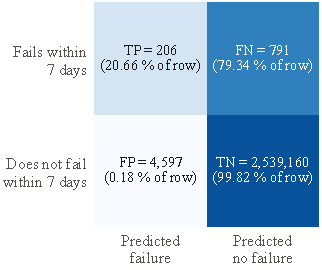
\includegraphics[width=0.8\columnwidth]{figures/g03_rf_confusion_matrix.pdf}
  \caption{\CapGZeroThreeRfConfusionMatrix}
  \label{fig:rf_cm}
\end{figure}

\begin{figure}[!t]
  \centering
  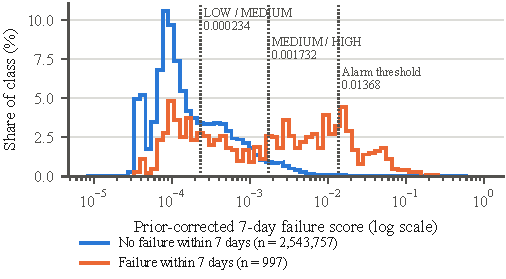
\includegraphics[width=\columnwidth]{figures/g04_rf_score_distribution.pdf}
  \caption{\CapGZeroFourRfScoreDistribution}
  \label{fig:rf_scores}
\end{figure}

\begin{figure*}[!t]
  \centering
  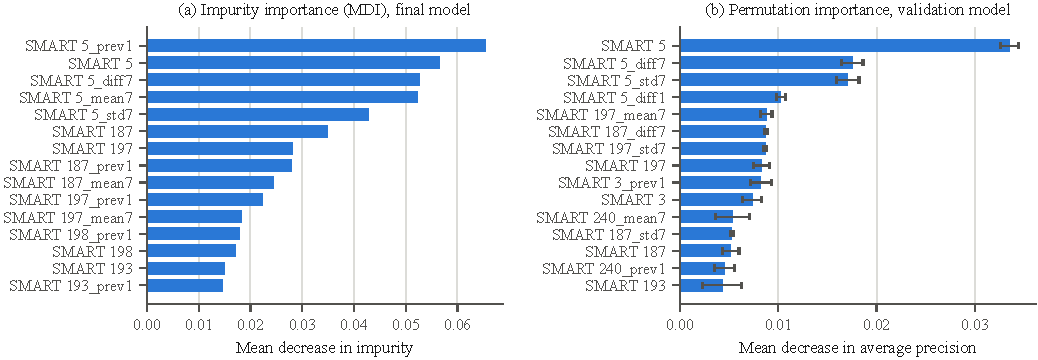
\includegraphics[width=\textwidth]{figures/g05_rf_feature_importance.pdf}
  \caption{\CapGZeroFiveRfFeatureImportance}
  \label{fig:rf_importance}
\end{figure*}

\begin{figure}[!t]
  \centering
  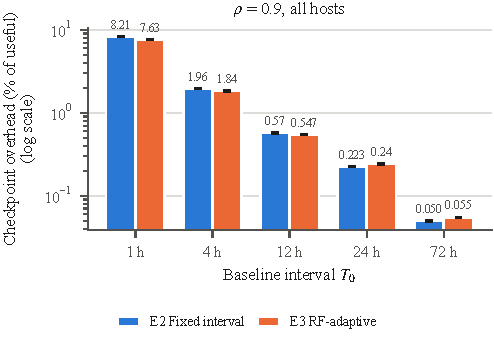
\includegraphics[width=\columnwidth]{figures/g06_overhead_vs_T0_rho09.pdf}
  \caption{\CapGZeroSixOverheadVsTZeroRhoZeroNine}
  \label{fig:overhead_rho09}
\end{figure}

\begin{figure}[!t]
  \centering
  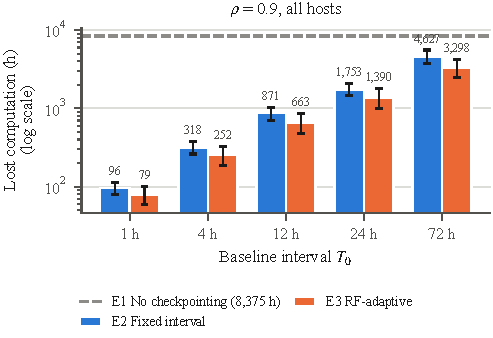
\includegraphics[width=\columnwidth]{figures/g07_lost_work_vs_T0_rho09.pdf}
  \caption{\CapGZeroSevenLostWorkVsTZeroRhoZeroNine}
  \label{fig:lost_rho09}
\end{figure}

\begin{figure}[!t]
  \centering
  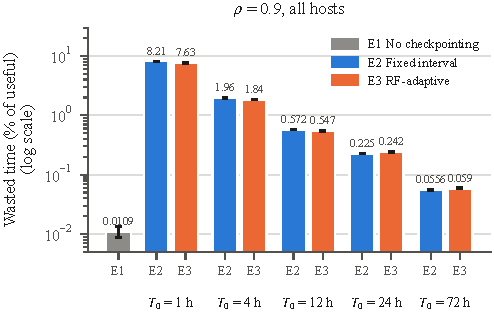
\includegraphics[width=\columnwidth]{figures/g09_wasted_time_all_policies_rho09.pdf}
  \caption{\CapGZeroNineWastedTimeAllPoliciesRhoZeroNine}
  \label{fig:wasted_rho09}
\end{figure}

\begin{figure}[!t]
  \centering
  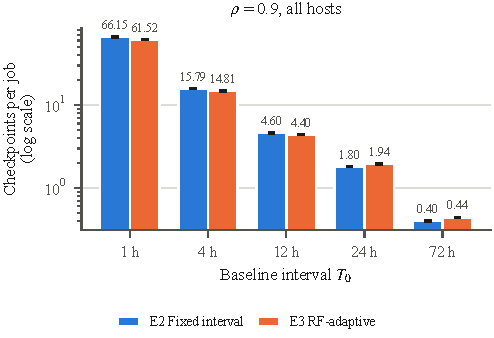
\includegraphics[width=\columnwidth]{figures/g11_checkpoints_per_job_rho09.pdf}
  \caption{\CapGElevenCheckpointsPerJobRhoZeroNine}
  \label{fig:ckpts_rho09}
\end{figure}

\begin{figure*}[!t]
  \centering
  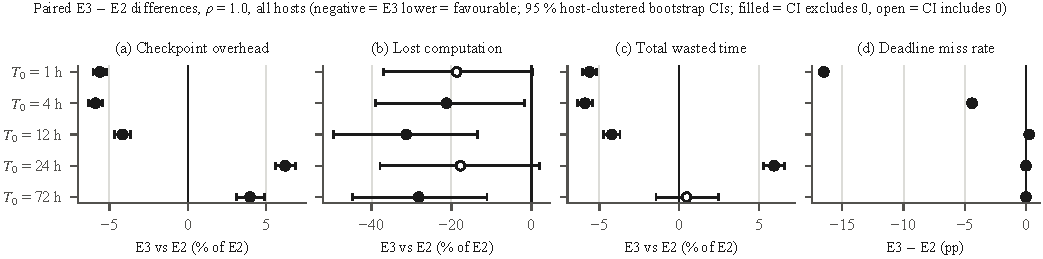
\includegraphics[width=\textwidth]{figures/g12_paired_E3_vs_E2_rho10.pdf}
  \caption{\CapGTwelvePairedEThreeVsETwoRhoOneZero}
  \label{fig:paired_rho10}
\end{figure*}

\begin{figure}[!t]
  \centering
  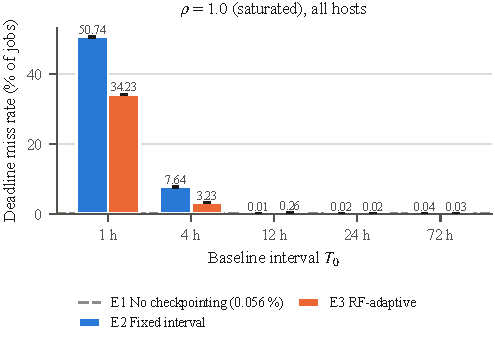
\includegraphics[width=\columnwidth]{figures/g13_deadline_miss_vs_T0_rho10.pdf}
  \caption{\CapGThirteenDeadlineMissVsTZeroRhoOneZero}
  \label{fig:deadline_rho10}
\end{figure}

\begin{figure}[!t]
  \centering
  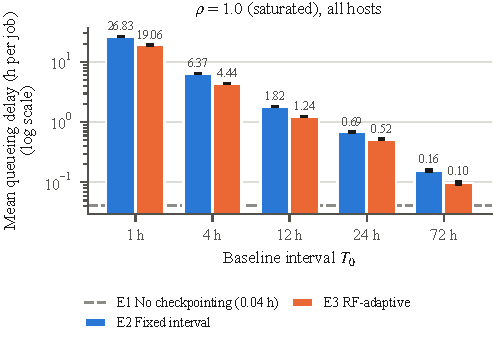
\includegraphics[width=\columnwidth]{figures/g14_queueing_vs_T0_rho10.pdf}
  \caption{\CapGFourteenQueueingVsTZeroRhoOneZero}
  \label{fig:queue_rho10}
\end{figure}

\begin{figure}[!t]
  \centering
  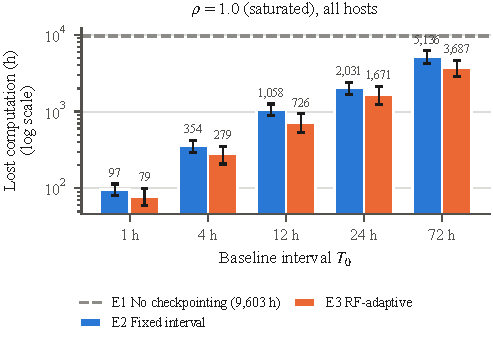
\includegraphics[width=\columnwidth]{figures/g15_lost_work_vs_T0_rho10.pdf}
  \caption{\CapGFifteenLostWorkVsTZeroRhoOneZero}
  \label{fig:lost_rho10}
\end{figure}

\begin{figure}[!t]
  \centering
  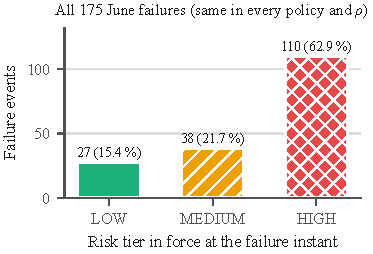
\includegraphics[width=0.8\columnwidth]{figures/g18_failures_by_tier.pdf}
  \caption{\CapGEighteenFailuresByTier}
  \label{fig:failures_tier}
\end{figure}

\begin{figure}[!t]
  \centering
  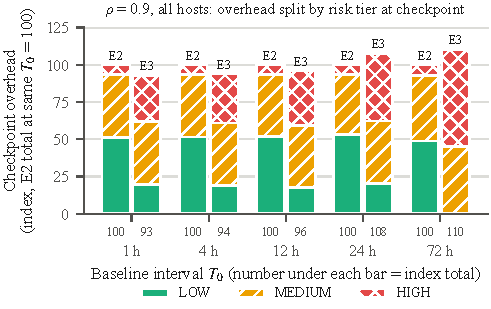
\includegraphics[width=\columnwidth]{figures/g20_overhead_by_tier_rho09.pdf}
  \caption{\CapGTwentyOverheadByTierRhoZeroNine}
  \label{fig:overhead_tier_rho09}
\end{figure}

% Auto-generated by paper_assets/scripts/make_tables.py from project/ml/processed/dataset_split_summary.csv, project/ml/preprocessing/config.py, project/ml/results/dataset_audit_revalidation/quality_excluded_drives.csv
\begin{table*}[!t]
\centering
\caption{Preprocessing and chronological split (7-day horizon).}
\label{tab:split}
\footnotesize
\setlength{\tabcolsep}{4pt}
\begin{tabular}{llrrrrrl}
\toprule
Period & Dates & Drive-days & Examples & Pos. rows & Pos. drives & Neg. rows & Use \\
\midrule
Train & 2019-04-01 -- 05-24 & 5,747,437 & 5,745,061 & 1,842 & 305 & 5,743,219 & model fitting (sampled 20 : 1) \\
Purge & 2019-05-25 -- 05-31 & 763,568 & 0 & 0 & 0 & 0 & gap; no examples \\
Test & 2019-06-01 -- 06-23 & 2,545,101 & 2,544,754 & 997 & 175 & 2,543,757 & single final evaluation; CloudSim scores \\
Tail & 2019-06-24 -- 06-30 & 774,849 & 0 & 0 & 0 & 0 & no 7-day follow-up; no examples \\
\bottomrule
\end{tabular}
\par\smallskip
\parbox{0.97\textwidth}{\scriptsize Positive: the drive records a failure on day t+1 \dots{} t+7. Primary negative: the drive is still observed on or after t+7; rows with shorter follow-up are excluded (censored). 5 drives with data-quality problems are excluded. Failure-day rows are not examples. Internal validation for model selection used 2019-04-01 -- 05-03 (fit), 05-04 -- 05-10 (purge), 05-11 -- 05-24 (validation), all inside the training period.}
\end{table*}

% Auto-generated by paper_assets/scripts/make_tables.py from project/ml/models/random_forest_7d_metadata.json, project/ml/training/rf_config.py
\begin{table}[!t]
\centering
\caption{Random Forest model configuration.}
\label{tab:rf_config}
\footnotesize
\setlength{\tabcolsep}{4pt}
\begin{tabular}{lp{0.56\columnwidth}}
\toprule
Parameter & Value \\
\midrule
Algorithm & Random Forest classifier (scikit-learn 1.7.2) \\
Prediction target & failure on day t+1 \dots{} t+7 given SMART history $\le$ t \\
Input features & 128 (no serial, date, model or capacity) \\
Trees / max features & 300 / sqrt \\
Max depth / min samples per leaf & 20 / 1 (selected) \\
Bootstrap / class weights & True / none \\
Missing values & kept as NaN (native routing) \\
Hyper-parameter grid & max depth {10, 20, none} $\times$ min leaf {1, 5, 20}; 9 configurations \\
Selection metric & PR-AUC on internal validation 2019-05-11 -- 2019-05-24 \\
Negative sampling & 20 : 1, stratified by date $\times$ model; 1,842 positives + 36,840 negatives \\
Prior correction & p = $\beta$s / ($\beta$s + 1 $-$ s), $\beta$ = 0.006415 \\
Alarm threshold (p) & 0.01368 (max F1 on validation) \\
Random seed & 20190401 \\
\bottomrule
\end{tabular}
\end{table}

% Auto-generated by paper_assets/scripts/make_tables.py from project/cloudsim/results/full_rho1.0/analysis/policy_summary.csv
\begin{table*}[!t]
\centering
\caption{Overall policy comparison, $\rho$ = 1.0 (saturated sensitivity).}
\label{tab:policy_rho10}
\footnotesize
\setlength{\tabcolsep}{4pt}
\begin{tabular}{lrrrrrrrrr}
\toprule
Policy & Miss \% & Lost (h) & Lost 95 \% CI & Overhead (h) & Ovh. \% & Waste \% & Queue h/job & Ckpt/job & Recov. (h) \\
\midrule
E1 none & 0.056 & 9,603 & [7,834, 11,500] & 0 & 0 & 0.011 & 0.042 & 0 & 8.75 \\
\midrule
E2 fixed, $T_0$ = 1 h & 50.74 & 96.77 & [81.27, 113.7] & 6,945,035 & 8.21 & 8.21 & 26.83 & 66.15 & 23.00 \\
E3 adaptive, $T_0$ = 1 h & 34.23 & 78.68 & [60.05, 99.45] & 6,554,774 & 7.75 & 7.75 & 19.06 & 62.43 & 23.08 \\
\midrule
E2 fixed, $T_0$ = 4 h & 7.64 & 354.0 & [293.8, 416.4] & 1,657,514 & 1.96 & 1.96 & 6.37 & 15.79 & 23.08 \\
E3 adaptive, $T_0$ = 4 h & 3.23 & 278.7 & [207.3, 352.9] & 1,559,670 & 1.84 & 1.84 & 4.44 & 14.85 & 22.83 \\
\midrule
E2 fixed, $T_0$ = 12 h & 0.011 & 1,058 & [878.9, 1,253] & 482,509 & 0.570 & 0.572 & 1.82 & 4.60 & 21.42 \\
E3 adaptive, $T_0$ = 12 h & 0.265 & 726.5 & [535.7, 932.9] & 462,438 & 0.547 & 0.548 & 1.24 & 4.40 & 21.92 \\
\midrule
E2 fixed, $T_0$ = 24 h & 0.024 & 2,031 & [1,683, 2,413] & 188,758 & 0.223 & 0.226 & 0.688 & 1.80 & 18.67 \\
E3 adaptive, $T_0$ = 24 h & 0.017 & 1,671 & [1,239, 2,128] & 200,507 & 0.237 & 0.239 & 0.522 & 1.91 & 20.17 \\
\midrule
E2 fixed, $T_0$ = 72 h & 0.042 & 5,136 & [4,232, 6,163] & 41,917 & 0.050 & 0.056 & 0.158 & 0.399 & 13.42 \\
E3 adaptive, $T_0$ = 72 h & 0.028 & 3,687 & [2,845, 4,688] & 43,586 & 0.052 & 0.056 & 0.098 & 0.415 & 17.17 \\
\bottomrule
\end{tabular}
\par\smallskip
\parbox{0.97\textwidth}{\scriptsize $\rho$ = 1.0, all 110,848 hosts, 1,259,916 jobs, 175 failures. Miss \% = late jobs / jobs. Lost = computation lost to failures. Overhead = 300 s $\times$ completed checkpoint writes (writes cut short by a failure are counted in Waste). Ovh. \% and Waste \% are percentages of useful compute (sum of job lengths); Waste = overhead + lost + interrupted writes + recovery. Queue = mean waiting time before a job starts. Lost-work CIs: paired host-clustered bootstrap (B = 2,000).}
\end{table*}

% Auto-generated by paper_assets/scripts/make_tables.py from project/cloudsim/results/full_rho1.0/analysis/policy_summary.csv
\begin{table*}[!t]
\centering
\caption{Failing versus non-failing hosts, $\rho$ = 1.0.}
\label{tab:strata_rho10}
\footnotesize
\setlength{\tabcolsep}{4pt}
\begin{tabular}{lrrrrrrrrr}
\toprule
 & \multicolumn{5}{c}{Failing hosts (175)} & \multicolumn{4}{c}{Non-failing hosts (110,673)} \\
\cmidrule(lr){2-6} \cmidrule(lr){7-10}
Policy & Miss \% & 95 \% CI & Lost (h) & Ovh. \% & Ckpt/job & Miss \% & Ovh. \% & Ckpt/job & Queue h/job \\
\midrule
E1 none & 35.66 & [31.31, 40.07] & 9,603 & 0 & 0 & 0 & 0 & 0 & 3.0e-05 \\
\midrule
E2 fixed, $T_0$ = 1 h & 51.48 & [49.12, 53.96] & 96.77 & 8.21 & 65.96 & 50.74 & 8.21 & 66.15 & 26.83 \\
E3 adaptive, $T_0$ = 1 h & 59.62 & [56.02, 63.06] & 78.68 & 11.53 & 92.68 & 34.19 & 7.74 & 62.38 & 19.02 \\
\midrule
E2 fixed, $T_0$ = 4 h & 14.87 & [12.91, 16.74] & 354.0 & 1.96 & 15.74 & 7.63 & 1.96 & 15.79 & 6.36 \\
E3 adaptive, $T_0$ = 4 h & 25.46 & [22.34, 28.52] & 278.7 & 3.07 & 24.67 & 3.20 & 1.84 & 14.84 & 4.42 \\
\midrule
E2 fixed, $T_0$ = 12 h & 6.68 & [4.55, 9.03] & 1,058 & 0.570 & 4.58 & 0 & 0.570 & 4.60 & 1.82 \\
E3 adaptive, $T_0$ = 12 h & 8.49 & [6.15, 11.05] & 726.5 & 0.973 & 7.82 & 0.252 & 0.546 & 4.40 & 1.23 \\
\midrule
E2 fixed, $T_0$ = 24 h & 15.22 & [12.41, 18.22] & 2,031 & 0.223 & 1.79 & 0 & 0.223 & 1.80 & 0.679 \\
E3 adaptive, $T_0$ = 24 h & 10.75 & [7.57, 14.47] & 1,671 & 0.435 & 3.50 & 0 & 0.237 & 1.91 & 0.511 \\
\midrule
E2 fixed, $T_0$ = 72 h & 26.27 & [22.44, 30.08] & 5,136 & 0.050 & 0.402 & 0 & 0.050 & 0.399 & 0.136 \\
E3 adaptive, $T_0$ = 72 h & 17.68 & [13.94, 21.89] & 3,687 & 0.118 & 0.946 & 0 & 0.051 & 0.414 & 0.079 \\
\bottomrule
\end{tabular}
\par\smallskip
\parbox{0.97\textwidth}{\scriptsize $\rho$ = 1.0. Failing hosts: the 175 hosts whose drive failed in June (one failure each); non-failing: 110,673 hosts. Non-failing hosts lose no work by construction. CI: host-clustered bootstrap within the stratum.}
\end{table*}

% Auto-generated by paper_assets/scripts/make_tables.py from project/cloudsim/results/full_rho0.9/analysis/failures_detail.csv, project/cloudsim/results/full_rho0.9/analysis/policy_summary.csv
\begin{table}[!t]
\centering
\caption{Lost computation by risk tier at failure, $\rho$ = 0.9.}
\label{tab:lost_tier_rho09}
\footnotesize
\setlength{\tabcolsep}{4pt}
\begin{tabular}{lrrrr}
\toprule
Policy & LOW & MEDIUM & HIGH & Total \\
\midrule
E1 none & 1,984.1 & 1,514.2 & 4,877.2 & 8,375.5 \\
\midrule
E2 fixed, $T_0$ = 1 h & 16.0 & 24.4 & 55.6 & 96.0 \\
E3 adaptive, $T_0$ = 1 h & 41.2 & 22.8 & 14.7 & 78.7 \\
\midrule
E2 fixed, $T_0$ = 4 h & 48.4 & 66.2 & 203.2 & 317.8 \\
E3 adaptive, $T_0$ = 4 h & 123.7 & 75.6 & 53.2 & 252.5 \\
\midrule
E2 fixed, $T_0$ = 12 h & 135.3 & 196.9 & 539.1 & 871.3 \\
E3 adaptive, $T_0$ = 12 h & 395.0 & 165.6 & 102.2 & 662.8 \\
\midrule
E2 fixed, $T_0$ = 24 h & 274.2 & 406.3 & 1,072.1 & 1,752.6 \\
E3 adaptive, $T_0$ = 24 h & 803.6 & 356.3 & 230.0 & 1,390.0 \\
\midrule
E2 fixed, $T_0$ = 72 h & 758.7 & 937.5 & 2,931.0 & 4,627.2 \\
E3 adaptive, $T_0$ = 72 h & 1,727.8 & 928.1 & 641.8 & 3,297.7 \\
\bottomrule
\end{tabular}
\par\smallskip
\parbox{0.97\columnwidth}{\scriptsize $\rho$ = 0.9. Lost computation (h) grouped by the risk tier in force at the failure instant (LOW n = 27, MEDIUM n = 38, HIGH n = 110 failures). Row totals equal the lost-work totals of the overall comparison. Point estimates only; with 27 -- 110 failures per tier, differences are uncertain.}
\end{table}

% Auto-generated by paper_assets/scripts/make_tables.py from project/cloudsim/results/full_rho1.0/analysis/failures_detail.csv, project/cloudsim/results/full_rho1.0/analysis/policy_summary.csv
\begin{table}[!t]
\centering
\caption{Lost computation by risk tier at failure, $\rho$ = 1.0.}
\label{tab:lost_tier_rho10}
\footnotesize
\setlength{\tabcolsep}{4pt}
\begin{tabular}{lrrrr}
\toprule
Policy & LOW & MEDIUM & HIGH & Total \\
\midrule
E1 none & 1,942.4 & 1,860.4 & 5,800.3 & 9,603.1 \\
\midrule
E2 fixed, $T_0$ = 1 h & 13.0 & 22.0 & 61.8 & 96.8 \\
E3 adaptive, $T_0$ = 1 h & 40.4 & 24.1 & 14.2 & 78.7 \\
\midrule
E2 fixed, $T_0$ = 4 h & 53.1 & 68.9 & 231.9 & 354.0 \\
E3 adaptive, $T_0$ = 4 h & 143.8 & 82.0 & 53.0 & 278.7 \\
\midrule
E2 fixed, $T_0$ = 12 h & 155.7 & 240.9 & 661.3 & 1,058.0 \\
E3 adaptive, $T_0$ = 12 h & 396.5 & 196.7 & 133.3 & 726.5 \\
\midrule
E2 fixed, $T_0$ = 24 h & 320.8 & 459.6 & 1,251.0 & 2,031.4 \\
E3 adaptive, $T_0$ = 24 h & 854.7 & 506.5 & 309.4 & 1,670.7 \\
\midrule
E2 fixed, $T_0$ = 72 h & 787.6 & 1,013.9 & 3,334.8 & 5,136.2 \\
E3 adaptive, $T_0$ = 72 h & 1,773.8 & 976.1 & 937.4 & 3,687.2 \\
\bottomrule
\end{tabular}
\par\smallskip
\parbox{0.97\columnwidth}{\scriptsize $\rho$ = 1.0. Lost computation (h) grouped by the risk tier in force at the failure instant (LOW n = 27, MEDIUM n = 38, HIGH n = 110 failures). Row totals equal the lost-work totals of the overall comparison. Point estimates only; with 27 -- 110 failures per tier, differences are uncertain.}
\end{table}

\bibliographystyle{IEEEtran}
\bibliography{references/references}
\end{document}
